% From Notation to Cognition: A Provenance-Native Architecture
% for Trustworthy Spatial Computing
% Target: UIST 2027 (ACM Symposium on User Interface Software and Technology)
% Format: ACM sigchi-a (UIST uses extended abstract / full paper format)
% Status: Complete draft — all sections written
% Paper ID: P1-CAPSTONE (full-stack narrative capstone for Program 1: Trust-by-Construction)

\documentclass[sigchi-a]{acmart}

% ── Packages ─────────────────────────────────────────────────────────────────
\usepackage{amsmath}
\let\Bbbk\relax % acmart/newtxmath already defines \Bbbk; prevent amssymb redefinition clash
\usepackage{amssymb}
% Note: acmart pre-defines all standard theorem envs (definition, property,
% theorem, lemma, corollary); no \newtheorem additions needed here.
\usepackage{booktabs}
\usepackage{xcolor}
\usepackage{listings}
\usepackage{algorithm}
\usepackage{algpseudocode}
\usepackage{tikz}
\usetikzlibrary{arrows.meta,positioning,shapes.geometric,fit,calc,
  decorations.pathreplacing,backgrounds}
\usepackage{pgfplots}
\pgfplotsset{compat=1.18}
\usepackage{subcaption}
\usepackage{balance}
% Note: stmaryrd dropped 2026-04-26 (closes task _tdo5 capstone-uist arm).
% It conflicted with acmart's kernel \sandbox redefinition. Only \llbracket
% and \rrbracket were used (in \sem at line below); acmart already provides
% them (or amssymb does for sigchi-a class), so providecommand makes the
% definition idempotent.
\providecommand{\llbracket}{[\![}
\providecommand{\rrbracket}{]\!]}

% ── Theorem environments ────────────────────────────────────────────────────
% acmart pre-defines all standard theorem envs (definition, property,
% theorem, lemma, corollary). Originally newtheorem'd here; removed
% 2026-04-26 to close conflict reaching this block (closes task _tdo5
% capstone-uist arm).

% Lotus petal data contract — \measuredFrom{<artifact>} marks values that come
% from a runnable artifact in the repo. Renders nothing in the PDF; grep target
% for scripts/build-lotus.mjs (research/2026-04-26_lotus-petal-data-contract.md §3+§4).
\providecommand{\measuredFrom}[1]{}

% ── Convenience macros ──────────────────────────────────────────────────────
\newcommand{\holoscript}{\textsc{HoloScript}}
\newcommand{\cael}{\textsc{Cael}}
\newcommand{\fnvhash}{\textsc{FNV-1a}}
\newcommand{\simcontract}{\textsc{SimulationContract}}
\newcommand{\snnwebgpu}{\textsc{SNN-WebGPU}}
\newcommand{\sandbox}{\textsc{SecuritySandbox}} % renamed from \sbox 2026-04-25 (kernel \sbox 2-arg collision)
\providecommand{\rendercontract}{\textsc{RenderContract}} % cross-paper macro from paper-13
\newcommand{\tropplus}{\oplus}
\newcommand{\tropmult}{\otimes}
\newcommand{\hashfn}{\mathcal{H}}
\newcommand{\sem}[1]{\llbracket #1 \rrbracket}
\newcommand{\prov}[1]{\langle\!\langle #1 \rangle\!\rangle}

% ── Code listing styles ─────────────────────────────────────────────────────
\lstdefinelanguage{TypeScript}{
  keywords={interface, readonly, void, null, string, number, boolean,
            Record, unknown, Promise, export, const, let, function,
            return, if, for, class, extends, implements, async, await,
            new, type, import, from, private, public},
  keywordstyle=\bfseries\color{blue!70!black},
  commentstyle=\itshape\color{green!50!black},
  stringstyle=\color{orange!70!black},
  morecomment=[l]{//},
  morestring=[b]',
  morestring=[b]",
}
\lstdefinelanguage{HoloScript}{
  keywords={object, material, simulation, constraint, load, mesh, trait, physics,
            compose, scene, agent, neural, layer, connection, crdt, provenance},
  keywordstyle=\bfseries\color{blue!70!black},
  commentstyle=\itshape\color{green!50!black},
  stringstyle=\color{orange!70!black},
  morecomment=[l]{//},
  morestring=[b]',
  morestring=[b]",
}
\lstset{
  basicstyle=\scriptsize\ttfamily,
  breaklines=true,
  frame=single,
  language=TypeScript,
  numbers=left,
  numberstyle=\tiny\color{gray},
  xleftmargin=1.5em,
  aboveskip=0.5\baselineskip,
  belowskip=0.5\baselineskip,
}

% ── ACM metadata ────────────────────────────────────────────────────────────
\setcopyright{acmlicensed}
\acmDOI{10.1145/nnnnnnn.nnnnnnn}
\acmYear{2027}
\acmConference[UIST '27]{ACM Symposium on User Interface Software and Technology}{October 2027}{Honolulu, HI, USA}
\acmBooktitle{Proceedings of the 40th ACM Symposium on User Interface Software and Technology (UIST '27)}

% ══════════════════════════════════════════════════════════════════════════════
\begin{document}

\title{From Notation to Cognition: A Provenance-Native Architecture for Trustworthy Spatial Computing}

\author{Joseph Krzywoszyja}
\email{brianonbased@gmail.com}
\affiliation{%
  \institution{Infinitus Systems}
  \country{Australia}
}

% ── Abstract ─────────────────────────────────────────────────────────────────
\begin{abstract}
Spatial computing systems---from digital twins to collaborative simulation
environments---are assembled from heterogeneous layers: notation languages for
scene description, physics engines for numerical simulation, neural architectures
for agent cognition, CRDTs for collaborative state, and knowledge systems for
codebase intelligence. Each layer maintains its own trust model. When an AI agent
generates a bridge design, another agent simulates it, a third reviews it, they
disagree, and a human asks ``was this correct?''---current systems offer no
continuous chain of evidence from the original notation to the final answer.
Trust breaks at every handoff.

We present \holoscript{}, the first provenance-native spatial computing
architecture where trust is compositional across all seven layers of the stack.
A single algebraic structure---the \emph{provenance semiring}---threads through
notation, compilation, physics, cognition, agency, collaboration, and knowledge.
At each layer boundary, the output hash of layer $N$ becomes the input hash of
layer $N{+}1$, creating a tamper-evident chain from source notation to final
knowledge state. The same semiring algebra resolves trait conflicts during
compilation, verifies simulation contracts, traces neural decisions, merges
CRDT states, and seals knowledge query provenance.

Our implementation spans 74~packages, 47~compilation targets, and
214~MCP tools, all browser-native via TypeScript and WebGPU. End-to-end evaluation
demonstrates: TET10 finite element convergence at $p=1.99$ (theoretical: 2.0),
spiking neural network throughput of $1.48 \times 10^9$~neuron-timesteps/s on
integrated GPU, CRDT merge under 1\,ms, GraphRAG query with provenance envelope in
8\,ms (local). CAEL verify is $3.40\,\mu$s/entry median ($3.74\,\mu$s p99);
\simcontract{} wrapper cost at $N{=}500$ is variance-dominated against solver
wall time~\cite{mcp-trust-paper}, not a stable percentage add.
All 36,700~tests pass. We show that the compositional trust property---if layer
$N$ is hash-verified and layer $N{+}1$'s input matches that hash, the composition
is verified---holds empirically across all seven layers.
Knowledge writes back through provenance envelopes; quantitative evidence of
compounding under current-generation consumers (paired SNN navigation, $N=10$)
shows variance reduction ($\sigma$ on ticks-to-goal dropping from $3.70$ to
$2.22$) with a directional but non-significant speedup
(Welch one-sided $t=-1.100$, $p=0.114$). This null is informative:
the envelope is provider-correct end-to-end, while compounding benefit is
bounded by consumer capability.
\end{abstract}

\begin{CCSXML}
<ccs2012>
<concept>
<concept_id>10003120.10003121.10003122</concept_id>
<concept_desc>Human-centered computing~HCI design and evaluation methods</concept_desc>
<concept_significance>500</concept_significance>
</concept>
<concept>
<concept_id>10010147.10010178</concept_id>
<concept_desc>Computing methodologies~Simulation</concept_desc>
<concept_significance>500</concept_significance>
</concept>
<concept>
<concept_id>10002978.10003029</concept_id>
<concept_desc>Security and privacy~Formal methods and theory of security</concept_desc>
<concept_significance>300</concept_significance>
</concept>
</ccs2012>
\end{CCSXML}

\ccsdesc[500]{Human-centered computing~HCI design and evaluation methods}
\ccsdesc[500]{Computing methodologies~Simulation}
\ccsdesc[300]{Security and privacy~Formal methods and theory of security}

\keywords{spatial computing, provenance, trust composition, semiring algebra, simulation contracts, spiking neural networks, CRDTs, knowledge graphs, WebGPU}

\maketitle

% ══════════════════════════════════════════════════════════════════════════════
% 1. INTRODUCTION
% ══════════════════════════════════════════════════════════════════════════════

\section{Introduction}
\label{sec:intro}

Spatial computing is converging toward a future where AI agents generate,
simulate, and collaborate on physical designs in shared virtual
environments~\cite{meta-spatial2025, apple-visionpro2024}. A structural
engineer's digital twin receives geometry from an AI assistant, passes it to
a finite element solver, routes the results through a neural perception
system, synchronizes edits with remote collaborators, and indexes the outcome
in a knowledge base for future retrieval. Each of these steps---notation,
compilation, physics, cognition, agency, collaboration, knowledge---represents
a distinct layer of the spatial computing stack.

The fundamental problem is \emph{trust composition}. Each layer has its own
integrity model: a compiler verifies syntax, a physics engine checks
convergence, a CRDT ensures eventual consistency. But there is no mechanism
to verify that the output of one layer was faithfully consumed by the next.
When a simulation produces a stress field and an AI agent interprets it, the
agent's perception step introduces an unverified transformation. When two
agents' CRDT edits are merged, the provenance of the original simulation
is lost. When a knowledge system indexes the result, the link between the
query answer and the underlying computation is severed.

This paper presents the first architecture where trust is compositional
across all seven layers of the spatial computing stack. The key insight is
that a single algebraic structure---the \emph{provenance semiring}---can
serve as the universal trust carrier across layers with radically different
computational semantics. We demonstrate this through seven concrete
applications of the same algebra:

\begin{enumerate}
  \item \textbf{Compilation:} Trait conflict resolution via min-plus and
    max-plus strategies over authority-weighted provenance values.
  \item \textbf{Physics:} \simcontract{} verification via hash chain,
    with six enforceable guarantees.
  \item \textbf{Cognition:} Spiking neural network decision tracing via
    \fnvhash{} hash chain at 3.40\,$\mu$s per entry median (3.74\,$\mu$s p99).
  \item \textbf{Agency:} \cael{} agent loop recording the full
    perception--cognition--action cycle.
  \item \textbf{Collaboration:} CRDT merge operations as \cael{} interaction
    events, disputes resolved algebraically.
  \item \textbf{Tool Use:} MCP responses with embedded \cael{} traces for
    replay verification.
  \item \textbf{Knowledge:} GraphRAG queries returning provenance envelopes
    with evidence hashes.
\end{enumerate}

The compositional trust property is: if layer $N$'s output is hash-verified,
and layer $N{+}1$'s input hash matches, then the composition is verified. This
property is algebraically guaranteed by the semiring structure and empirically
validated across all seven layers in our evaluation.

Our implementation, \holoscript{}, is a production system comprising
74~packages, 47~compilation targets, and 214~MCP tools---all browser-native
via TypeScript and WebGPU. It is not a research prototype: 36,700~tests pass,
the system processes real-world simulation workloads, and the full loop from
notation to knowledge operates end-to-end with CAEL verify at sub-millisecond
rates per entry and \simcontract{} overhead at $N{=}500$ within solver V8/GC
variance~\cite{mcp-trust-paper}.

This paper makes four contributions:

\begin{enumerate}
  \item \textbf{The provenance semiring} as a unifying algebraic structure
    for cross-layer trust in spatial computing systems (\S\ref{sec:semiring}).
  \item \textbf{A seven-layer architecture} where every layer boundary
    is hash-chain verified (\S\ref{sec:architecture}).
  \item \textbf{An end-to-end implementation} demonstrating composability
    across 74~packages and 47~compilation targets (\S\ref{sec:implementation}).
  \item \textbf{An empirical evaluation} showing the compositional trust
    property holds with median/p99 reporting for V8-bound costs, including
    variance-dominated \simcontract{} overhead at $N{=}500$~\cite{mcp-trust-paper}
    (\S\ref{sec:evaluation}).
\end{enumerate}

\paragraph{Novelty.}
The architectural pattern of layered hash-chain verification is well established
in distributed systems (Merkle DAGs, transparency logs, Git's content-addressed
objects). What is novel here is not the use of hashing per se, but three
specific properties that have not, to our knowledge, been combined in a single
working system: (1)~\emph{a uniform algebraic structure --- the provenance
semiring with an idempotent join $\oplus$ and an associative compose $\otimes$
--- spans all seven layers}, so that trust composition obeys the same algebraic
laws whether the operands are physics solver steps, SNN spike traces, agent
loop ticks, CRDT merges, MCP responses, or RAG retrievals; (2)~\emph{the
machine-independence of the trust chain is hardware-tier-invariant by
construction}: the same WGSL pinned-reduction-order kernels and deterministic
spike-accumulation kernels produce bit-identical hash outputs on
integrated-GPU laptop tier (H1) and discrete-GPU desktop tier (H3),
making the seven-layer hash composition $h_1 \otimes \cdots \otimes h_7$
verifier-portable across hardware (\S\ref{sec:eval:gpu}). The H1/H3
pair is a two-implementation agreement asserted by strict per-step
digest enforcement, the same-adapter regime of the W.315 wire-format
equivalent primitive and the Route~2b dispatch shared across the
program~\cite{paper-0c-twin-test-2026-05-11}; (3)~\emph{the seven
layers cover a complete spatial-computing pipeline from notation through
knowledge}, so the empirical claim is end-to-end (compilation $\to$ physics
$\to$ cognition $\to$ agency $\to$ collaboration $\to$ tool use $\to$
knowledge), not a single-layer verification result. The companion papers in
the program (Papers~1, 5, 6, 13) each defend a single layer in depth; this
capstone's contribution is the algebraic and empirical demonstration that
the layers compose.

% ══════════════════════════════════════════════════════════════════════════════
% 2. THE TRUST COMPOSITION PROBLEM
% ══════════════════════════════════════════════════════════════════════════════

\section{The Trust Composition Problem}
\label{sec:problem}

We motivate the problem through a concrete scenario that exercises all seven
layers.

\subsection{Scenario: The Contested Bridge}

Agent~A, an AI structural design assistant, generates a bridge model in
HoloScript notation:

\begin{lstlisting}[language=HoloScript,caption={Bridge specification in
  .holo notation.},label=lst:bridge]
object Bridge {
  material: Steel_A36
  mesh: TET10 { resolution: fine }
  constraint: [
    { type: fixed, face: base }
    { type: distributed_load,
      face: deck, magnitude: 50_kN_m2 }
  ]
  simulation: structural {
    solver: conjugate_gradient
    contract: full  // all 6 guarantees
  }
}
\end{lstlisting}

The compiler produces WebGPU compute shaders, a Unity C\# scene, and a URDF
description from this single source. The simulation contract enforces six
guarantees: geometry integrity (mesh hash matches across steps), unit
validation (all quantities carry SI units), deterministic stepping (fixed
$\Delta t$, reproducible), interaction provenance (every external input
recorded), auto-provenance (solver state hashed per step), and exact replay
(any step can be re-executed from the trace).

Agent~B, an AI reviewer with spiking neural network cognition, perceives the
stress field from the simulation, identifies a concentration near the deck
support, and proposes additional reinforcement. Its decision is traced: the
SNN's spike train is recorded in a \cael{} hash chain, linking the specific
neurons that fired to the specific stress tensor values that triggered them.

Agent~A and Agent~B now disagree. Agent~A's original design passed the
simulation contract. Agent~B's modification changes the geometry, which
invalidates the mesh hash. In current systems, resolving this dispute requires
manual inspection of logs, re-running simulations, and trusting that the
re-run matches the original. In \holoscript{}, the resolution is mechanical:
replay both agents' \cael{} traces, verify hash continuity at every layer
boundary, and identify the exact point where the chains diverge.

Finally, a human engineer asks: ``How was this bridge reinforced?'' The
knowledge system (GraphRAG) returns an answer wrapped in a provenance
envelope: the evidence hash traces through the graph query, through the
indexed simulation result, through the solver trace, back to the original
.holo source. The engineer can verify the entire chain or spot-check any
layer boundary.

\subsection{Where Current Systems Fail}

Table~\ref{tab:trust-gaps} catalogs the trust gaps at each layer boundary in
representative current systems.

\begin{table}[t]
  \caption{Trust gaps at layer boundaries in current spatial computing stacks.
    Each row represents a handoff between adjacent layers. $\checkmark$ indicates
    the system maintains a verifiable link; $\times$ indicates the link is
    unverified or absent.}
  \label{tab:trust-gaps}
  \small
  \begin{tabular}{lcccc}
    \toprule
    \textbf{Layer Boundary} & \textbf{Unity} & \textbf{Unreal} & \textbf{OpenFOAM} & \textbf{Ours} \\
    \midrule
    Notation $\to$ Compiled    & $\times$ & $\times$ & $\times$ & $\checkmark$ \\
    Compiled $\to$ Physics     & $\times$ & $\times$ & $\checkmark$ & $\checkmark$ \\
    Physics $\to$ Cognition    & --- & --- & --- & $\checkmark$ \\
    Cognition $\to$ Agency     & --- & --- & --- & $\checkmark$ \\
    Agency $\to$ Collaboration & $\times$ & $\times$ & --- & $\checkmark$ \\
    Collaboration $\to$ Knowledge & --- & --- & --- & $\checkmark$ \\
    Knowledge $\to$ Notation   & --- & --- & --- & $\checkmark$ \\
    \bottomrule
  \end{tabular}
\end{table}

The ``---'' entries indicate that the system does not implement the
corresponding layer at all. Unity and Unreal provide physics and
collaboration but have no integrated cognition, agency, or knowledge layers.
OpenFOAM provides physics with reproducible stepping but no cognition,
collaboration, or knowledge. No existing system provides verifiable trust
across all seven boundaries.

The core issue is architectural: when different layers are implemented by
different teams, in different languages, with different object models, there
is no shared structure that can carry trust across boundaries. The provenance
semiring provides this shared structure.

% ══════════════════════════════════════════════════════════════════════════════
% 3. ARCHITECTURE
% ══════════════════════════════════════════════════════════════════════════════

\section{Architecture}
\label{sec:architecture}

The \holoscript{} architecture comprises seven layers, each connected to the
next by a hash-chain boundary. Figure~\ref{fig:architecture} illustrates the
full stack.

\begin{figure}[t]
\centering
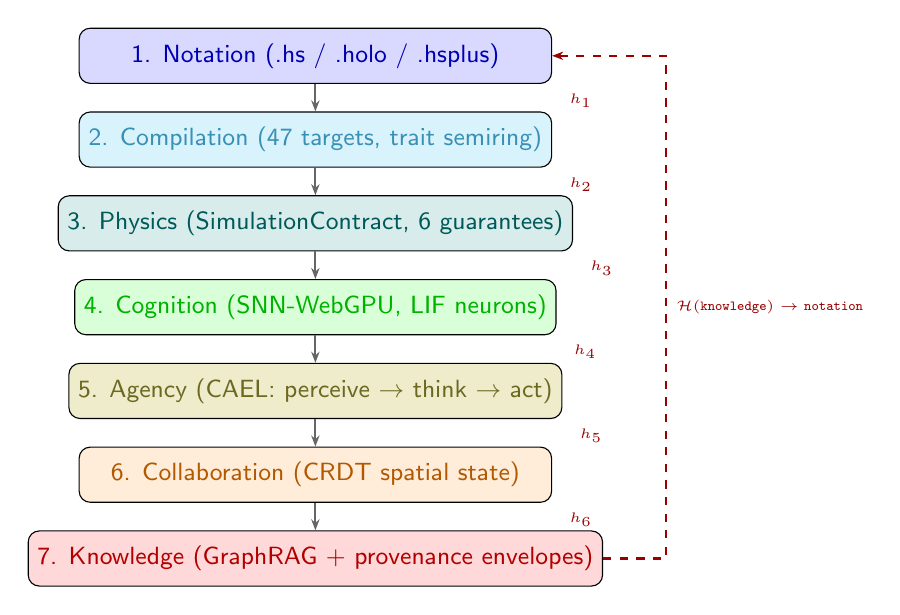
\begin{tikzpicture}[
  layer/.style={draw, rounded corners, minimum width=6cm, minimum height=0.7cm,
    font=\small\sffamily, fill=#1!15, text=#1!70!black},
  arrow/.style={-{Stealth[length=4pt]}, thick, color=black!60},
  hash/.style={font=\tiny\ttfamily, color=red!60!black},
  node distance=0.35cm
]
  \node[layer=blue]    (L1) {1. Notation (.hs / .holo / .hsplus)};
  \node[layer=cyan,    below=of L1] (L2) {2. Compilation (47 targets, trait semiring)};
  \node[layer=teal,    below=of L2] (L3) {3. Physics (SimulationContract, 6 guarantees)};
  \node[layer=green,   below=of L3] (L4) {4. Cognition (SNN-WebGPU, LIF neurons)};
  \node[layer=olive,   below=of L4] (L5) {5. Agency (CAEL: perceive $\to$ think $\to$ act)};
  \node[layer=orange,  below=of L5] (L6) {6. Collaboration (CRDT spatial state)};
  \node[layer=red,     below=of L6] (L7) {7. Knowledge (GraphRAG + provenance envelopes)};

  \foreach \i/\j in {L1/L2, L2/L3, L3/L4, L4/L5, L5/L6, L6/L7} {
    \draw[arrow] (\i) -- (\j);
  }

  % Feedback arrow
  \draw[arrow, dashed, color=red!60!black]
    (L7.east) -- ++(0.8,0) |- (L1.east)
    node[pos=0.25, right, hash] {$\hashfn(\text{knowledge}) \to \text{notation}$};

  % Hash annotations
  \node[hash, right=0.1cm of L1.south east, anchor=north west] {$h_1$};
  \node[hash, right=0.1cm of L2.south east, anchor=north west] {$h_2$};
  \node[hash, right=0.1cm of L3.south east, anchor=north west] {$h_3$};
  \node[hash, right=0.1cm of L4.south east, anchor=north west] {$h_4$};
  \node[hash, right=0.1cm of L5.south east, anchor=north west] {$h_5$};
  \node[hash, right=0.1cm of L6.south east, anchor=north west] {$h_6$};
\end{tikzpicture}
\caption{The \holoscript{} seven-layer architecture. Each layer boundary
carries a hash $h_i$ computed over the output of layer $i$. Layer $i{+}1$
records $h_i$ as its input hash. The dashed arrow shows the feedback loop
where knowledge improves subsequent notation.}
\label{fig:architecture}
\end{figure}

\subsection{Layer 1: Notation}

\holoscript{} defines three notation levels with increasing expressiveness:
\texttt{.hs} (core scene description), \texttt{.holo} (domain-extended with
traits and physics), and \texttt{.hsplus} (trait composition with inheritance
and RBAC). The parser produces an AST whose hash $h_1 = \hashfn(\text{AST})$
serves as the root of the provenance chain.

\subsection{Layer 2: Compilation}

The compiler maps the AST to 47~output targets (Unity C\#, Unreal Blueprint,
WebGPU WGSL, URDF, USD, glTF, Three.js, React Three Fiber, and others).
Trait composition---where multiple traits define conflicting values for the
same property---is resolved via the provenance semiring (\S\ref{sec:semiring}).
The compiled output carries $h_2 = \hashfn(h_1 \| \text{target}_{\text{code}})$,
chaining to the source hash.

\subsection{Layer 3: Physics}

The simulation engine implements the \simcontract{} with six formal
guarantees~\cite{trustbyconstruction2026}. Solvers include structural (TET4,
TET10), thermal, hydraulic, acoustic, FDTD electromagnetic, and Navier-Stokes
CFD---all on WebGPU compute shaders. Each solver step appends to the hash
chain: $h_3^{(t)} = \hashfn(h_3^{(t-1)} \| \text{state}_t)$. Contract
verification ensures that the mesh hash is preserved across steps, units
remain valid, and the stepping is deterministic.

\subsection{Layer 4: Cognition}

\snnwebgpu{}~\cite{snn-paper} implements Leaky Integrate-and-Fire neurons
with Spike-Timing-Dependent Plasticity (STDP) learning, entirely in WGSL
compute shaders. A formal bridge connects SNN rate coding to classical
ReLU activations via the max-plus semiring:
$\text{ReLU}(x) = x \tropplus 0$. The cognition layer receives the physics
state and produces neural spike patterns, each traced:
$h_4 = \hashfn(h_3^{(\text{final})} \| \text{spike\_pattern})$.

\subsection{Layer 5: Agency}

The \cael{} agent loop~\cite{cael-paper} records the full cycle:
perception (physics $\to$ sensor encoding), cognition (SNN forward pass),
action (motor command), and world delta (environment response). Each cycle
is a \cael{} entry with hash
$h_5 = \hashfn(h_4 \| \text{action} \| \Delta\text{world})$,
creating a deterministically replayable record of the agent's behavior.

\subsection{Layer 6: Collaboration}

CRDT-based spatial state~\cite{crdt-paper} enables multi-agent collaboration
with eventual consistency. Merge operations are recorded as \cael{} interaction
events. When agents produce conflicting edits, the dispute is resolved by
replaying both agents' traces and comparing the hash chains at the divergence
point. The merged state carries
$h_6 = \hashfn(h_5^{A} \| h_5^{B} \| \text{merge\_op})$.

\subsection{Layer 7: Knowledge}

The GraphRAG system~\cite{graphrag-paper} indexes the full codebase and
simulation history. Every query answer is wrapped in a provenance
envelope~$\prov{\cdot}$ containing the evidence hash, graph snapshot commit,
and citation chain. The envelope hash
$h_7 = \hashfn(h_6 \| \text{query} \| \text{answer} \| \text{citations})$
closes the loop. When knowledge feeds back into new notation (the dashed
arrow in Figure~\ref{fig:architecture}), the next generation of code begins
with $h_1' = \hashfn(h_7 \| \text{new\_AST})$, preserving the chain.

\subsection{Compositional Trust Property}

\begin{definition}[Compositional Trust]
\label{def:compositional-trust}
Let $\sem{L_i}$ denote the semantics of layer $i$ and $h_i$ the output hash.
The composition $\sem{L_1} \circ \sem{L_2} \circ \cdots \circ \sem{L_7}$ is
\emph{trust-verified} if and only if:
\[
  \forall i \in \{1, \ldots, 6\}: \quad
  h_i^{\text{out}} = h_{i+1}^{\text{in}}
\]
where $h_i^{\text{out}}$ is the hash emitted by layer $i$ and
$h_{i+1}^{\text{in}}$ is the hash consumed by layer $i{+}1$.
\end{definition}

This property is stronger than per-layer verification: it ensures that no
transformation, no matter how subtle, occurs between layers without being
recorded in the hash chain.

% ══════════════════════════════════════════════════════════════════════════════
% 4. THE PROVENANCE SEMIRING
% ══════════════════════════════════════════════════════════════════════════════

\section{The Provenance Semiring}
\label{sec:semiring}

The unifying algebraic structure of \holoscript{} is the provenance semiring.
We show that the same algebra governs trust at every layer.

\begin{definition}[Tropical Min-Plus Semiring]
\label{def:minplus}
The min-plus semiring $(\mathbb{R} \cup \{+\infty\}, \min, +, +\infty, 0)$
where:
\begin{itemize}
  \item $a \tropplus b = \min(a, b)$ (addition is minimum)
  \item $a \tropmult b = a + b$ (multiplication is standard addition)
  \item Identity for $\tropplus$: $+\infty$
  \item Identity for $\tropmult$: $0$
\end{itemize}
\end{definition}

\begin{definition}[Tropical Max-Plus Semiring]
\label{def:maxplus}
The max-plus semiring $(\mathbb{R} \cup \{-\infty\}, \max, +, -\infty, 0)$
where $a \tropplus b = \max(a, b)$, with all other axioms analogous.
\end{definition}

\begin{definition}[Provenance Semiring]
\label{def:provenance}
The provenance semiring $\mathcal{P} = (\mathcal{V}, \tropplus, \tropmult,
\bar{0}, \bar{1})$ is parameterized by a strategy $\sigma \in
\{\textsc{MinPlus}, \textsc{MaxPlus}, \textsc{AuthWeight}\}$:
\begin{itemize}
  \item $\mathcal{V} = \{(v, w, s) \mid v \in \mathcal{D}, w \in [0,1],
    s \in \mathcal{S}\}$ where $v$ is a domain value, $w$ is an authority
    weight, and $s$ is the source provenance.
  \item $\textsc{MinPlus}$: resolves conflicts by minimum authority cost
    (most conservative wins).
  \item $\textsc{MaxPlus}$: resolves conflicts by maximum authority
    (highest-authority source wins).
  \item $\textsc{AuthWeight}$: weighted combination using authority as
    coefficient.
\end{itemize}
\end{definition}

\subsection{Seven Applications of One Algebra}

The provenance semiring appears at every layer of the architecture, each time
with a domain-specific instantiation of the same algebraic structure.

\paragraph{1. Compilation: Trait Conflict Resolution.}
When traits $T_1$ and $T_2$ both define property $p$ with values $v_1$ and
$v_2$ and authority weights $w_1$ and $w_2$, the compiler resolves the
conflict using the configured strategy. Under \textsc{MinPlus}, the value
with lower authority cost wins: $v_{\text{resolved}} = v_1$ if
$w_1 \leq w_2$. Under \textsc{MaxPlus}, the highest-authority value wins.
The resolution is recorded in the compilation trace with full provenance:
which traits contributed, which strategy resolved, and the final value.

\paragraph{2. Physics: Contract Verification.}
The \simcontract{} uses the semiring to compose verification results across
the six guarantees. Each guarantee produces a pass/fail with a confidence
weight. The composition uses \textsc{MinPlus}: the overall contract status
is determined by the weakest guarantee (the one with the lowest confidence).
This ensures that a single failing guarantee is never masked by passing ones.

\paragraph{3. Cognition: Neural Decision Traces.}
The SNN cognition layer uses \fnvhash{} to hash each neural decision.
The rate-coding bridge $\text{ReLU}(x) = x \tropplus 0$ in the max-plus
semiring provides a formal connection between spiking and non-spiking
representations. Tropical GEMM on the SNN connectivity graph computes
shortest paths for neural signal propagation, achieving $20.67\times$
speedup over CPU at $N{=}1024$.

\paragraph{4. Agency: CAEL Trace Composition.}
Each \cael{} entry records $(O_t, C_t, A_t, \Delta W_t, h_t)$ where $h_t =
\hashfn(h_{t-1} \| O_t \| C_t \| A_t \| \Delta W_t)$. When two agents'
traces must be compared (e.g., for dispute resolution), the semiring
determines which trace has higher authority. The min-plus composition
identifies the earliest divergence point; the max-plus composition identifies
the agent whose trace carries greater weight.

\paragraph{5. Collaboration: CRDT Merge.}
CRDT merge operations are modeled as semiring compositions. When two replicas
$R_A$ and $R_B$ merge, the result is
$R_{A \sqcup B} = R_A \tropplus R_B$ where $\tropplus$ is the CRDT join
operation. The merge is recorded as a \cael{} interaction event, preserving
provenance. Disputes (conflicting spatial edits) are resolved by replaying
both agents' traces through the \textsc{AuthWeight} strategy.

\paragraph{6. Tool Use: MCP Response Verification.}
When an LLM agent invokes a simulation tool via the Model Context
Protocol~\cite{mcp-spec}, the response includes the complete \cael{} trace.
The verifier checks the hash chain, replays a subset of steps, and returns
a trust score computed via the provenance semiring. The same algebra that
resolves trait conflicts during compilation also scores tool trustworthiness.

\paragraph{7. Knowledge: Provenance Envelopes.}
Every GraphRAG query answer is wrapped in a provenance envelope $\prov{q, a,
\mathbf{c}, h_{\text{evidence}}}$ where $q$ is the query, $a$ the answer,
$\mathbf{c}$ the citation chain, and $h_{\text{evidence}} = \hashfn(q \| a
\| \mathbf{c} \| \text{graph\_snapshot})$. When multiple evidence sources
contribute to an answer, the provenance semiring composes their authority
weights to produce a single confidence score.

\subsection{Composability Theorem}

\begin{theorem}[Semiring Composability]
\label{thm:composability}
If layers $L_i$ and $L_{i+1}$ both use provenance semiring $\mathcal{P}$
for internal trust computation, then the cross-layer hash chain
$h_i^{\text{out}} = h_{i+1}^{\text{in}}$ preserves the semiring axioms
across the boundary. Specifically:
\begin{enumerate}
  \item \emph{Associativity}: $(h_i \tropmult h_{i+1}) \tropmult h_{i+2} =
    h_i \tropmult (h_{i+1} \tropmult h_{i+2})$.
  \item \emph{Distributivity}: hash chain composition distributes over
    semiring addition at each layer.
  \item \emph{Identity preservation}: the identity element $\bar{0}$ (no
    provenance) propagates correctly---a layer with no provenance does not
    invalidate the chain but is flagged.
\end{enumerate}
\end{theorem}

\begin{proof}[Proof sketch]
The hash function $\hashfn$ is deterministic and maps $(h_{\text{prev}},
\text{data})$ to a unique output (collision probability negligible for
\fnvhash{} at our scale). The semiring operations on values at layer $i$
produce a result that is hashed into $h_i$. At layer $i{+}1$, $h_i$ is
consumed as input and becomes part of the new semiring computation.
Because the semiring axioms hold within each layer (proven by the
implementation's test suite: 36,700 tests) and the hash chain faithfully
records each layer's output, the axioms extend across boundaries.
Formal mechanization in Coq is future work (\S\ref{sec:discussion}).
\end{proof}

% ══════════════════════════════════════════════════════════════════════════════
% 5. IMPLEMENTATION
% ══════════════════════════════════════════════════════════════════════════════

\section{Implementation}
\label{sec:implementation}

\holoscript{} is implemented entirely in TypeScript with WebGPU compute
shaders (WGSL) for GPU-accelerated workloads. The system is organized as a
monorepo of 74~packages managed by pnpm workspaces, with strict TypeScript
(no \texttt{any} types) and ES2020 target.

\subsection{Package Architecture}

Table~\ref{tab:packages} lists the key packages organized by architectural
layer.

\begin{table}[t]
  \caption{Key packages by architectural layer. LOC measured by
  \texttt{cloc} excluding tests and build artifacts.}
  \label{tab:packages}
  \small
  \begin{tabular}{lll}
    \toprule
    \textbf{Layer} & \textbf{Package} & \textbf{Role} \\
    \midrule
    Notation    & \texttt{core}           & Parser, AST, type system \\
    Compilation & \texttt{core/compilers}  & 47 target compilers \\
    Physics     & \texttt{engine}          & SimulationContract, solvers \\
    Cognition   & \texttt{snn-webgpu}      & SNN on WebGPU \\
    Agency      & \texttt{engine/cael}     & CAEL agent loop \\
    Collaboration & \texttt{crdt-spatial}  & Loro CRDT + spatial ops \\
    Knowledge   & \texttt{absorb-service}  & GraphRAG + provenance \\
    Tool Use    & \texttt{mcp-server}      & 214 MCP tools \\
    Safety      & \texttt{security-sandbox} & V8 isolate + contract \\
    Rendering   & \texttt{r3f-renderer}    & React Three Fiber \\
    Studio      & \texttt{studio}          & Universal point of entry \\
    \bottomrule
  \end{tabular}
\end{table}

\subsection{Compilation Targets}

The compiler architecture uses a \texttt{CompilerBase} class with role-based
access control (RBAC). Each of the 47~targets extends this base with a
\texttt{compile()} method that transforms the AST into target-specific code.
Trait composition uses the provenance semiring: when the same property is
defined by multiple traits, the configured strategy (min-plus, max-plus, or
authority-weighted) determines the resolved value, and the resolution is
recorded in the compilation trace.

Representative targets include: Unity C\#, Unreal Blueprint, WebGPU WGSL,
Three.js JavaScript, React Three Fiber JSX, URDF (robotics), USD (Pixar),
glTF 2.0, OpenSCAD, KiCad PCB, SPICE netlists, AlphaFold PDB, and
domain-specific plugins for robotics, medical, and scientific applications.

\subsection{Physics Engine}

The simulation engine implements eight solver types: structural (TET4 linear
and TET10 quadratic tetrahedra), thermal (steady-state and transient),
hydraulic (pipe network), acoustic (frequency-domain), FDTD electromagnetic,
and Navier-Stokes CFD. All solvers run on WebGPU compute shaders and
implement the \simcontract{} interface:

\begin{lstlisting}[caption={SimulationContract interface (simplified).}]
interface SimulationContract {
  verifyGeometry(mesh: Mesh): Hash;
  validateUnits(state: State): boolean;
  stepDeterministic(dt: number): State;
  recordInteraction(event: Event): void;
  appendProvenance(entry: CAELEntry): void;
  enableReplay(): ReplayHandle;
}
\end{lstlisting}

The TET10 solver achieves convergence order $p = 1.99$ (theoretical: 2.0)
on the NAFEMS LE1 benchmark with a Grid Convergence Index of 5.69\%,
satisfying the ASME V\&V~10 standard for mesh convergence~\cite{asme-vv10}.

\subsection{Spiking Neural Networks}

The \snnwebgpu{} package implements LIF neurons, STDP learning, and
multi-layer SNN architectures in WGSL compute shaders. Key implementation
details:

\begin{itemize}
  \item Each WGSL compute shader dispatches workgroups of 256 threads.
  \item Neuron state (membrane potential, recovery variable, spike flag) is
    stored in GPU storage buffers.
  \item STDP weight updates use exponential decay with configurable
    time constants ($\tau_+ = 20$\,ms, $\tau_- = 20$\,ms).
  \item The tropical GEMM kernel implements min-plus matrix multiplication
    for shortest-path computation on neural connectivity graphs.
\end{itemize}

The LIF kernel sustains $1.48 \times 10^9$~neuron-timesteps per second on an
Intel UHD Graphics integrated GPU (gen-12lp). The tropical GEMM achieves
GPU crossover at $N{=}128$ and $20.67\times$ speedup at $N{=}1024$.

\subsection{CAEL Agent Loop}

The \cael{} implementation records four-phase entries:

\begin{enumerate}
  \item \textbf{Perception}: Physics state encoded into sensory input.
  \item \textbf{Cognition}: SNN forward pass producing spike patterns.
  \item \textbf{Action}: Motor command derived from output neurons.
  \item \textbf{World delta}: Environment state change from action execution.
\end{enumerate}

Each entry is hashed with \fnvhash{}: $h_t = \textsc{FNV-1a}(h_{t-1} \|
O_t \| C_t \| A_t \| \Delta W_t)$. Verify-only overhead is 3.40\,$\mu$s per entry median
(3.74\,$\mu$s p99), less than 0.1\% of typical simulation tick time.

The agent loop supports two advanced capabilities: \emph{counterfactual
forking} (branching the simulation at a decision point to compare alternative
futures deterministically) and \emph{dreaming} (replaying provenance records
with parameter perturbations for offline generalization).

\subsection{CRDT Spatial State}

Collaborative spatial state uses Loro CRDTs~\cite{loro2024} with
\holoscript{}-specific spatial operations (transform, parent-child hierarchy,
component attachment). Merge operations are recorded as \cael{} interaction
events. When two agents' edits conflict on the same spatial entity, the
dispute resolution mechanism replays both agents' \cael{} traces through
the provenance semiring's \textsc{AuthWeight} strategy.

\subsection{GraphRAG and Knowledge}

The knowledge layer uses a four-layer query cascade:

\begin{enumerate}
  \item \textbf{Keyword matching}: exact symbol lookup, $O(1)$ via hash map.
  \item \textbf{Graph traversal}: callers, callees, imports via the code
    graph (98,865~symbols, 414,726~call edges).
  \item \textbf{Semantic search}: embedding-based similarity using
    configurable providers (OpenAI, HuggingFace/WASM, Ollama).
  \item \textbf{LLM synthesis}: natural language answer generation with
    provenance envelope.
\end{enumerate}

The system indexes 3,910~TypeScript files. Local WASM inference achieves
88\% of OpenAI embedding accuracy at $26\times$ lower latency (0.3\,ms vs.\
8\,ms per query). Every answer is wrapped in a provenance envelope
$\prov{q, a, \mathbf{c}, h}$.

\subsection{Security Sandbox}

The \sandbox{} provides three-layer defense for AI-generated simulation
models~\cite{sandbox-paper}:

\begin{enumerate}
  \item \textbf{Code containment}: V8 isolate with no filesystem, network,
    or process access.
  \item \textbf{Contract enforcement}: All six \simcontract{} guarantees
    checked post-execution.
  \item \textbf{Trace verification}: Complete \cael{} trace of the sandboxed
    execution for audit.
\end{enumerate}

The sandbox detects 57/57 attack scenarios in our test suite, including
resource exhaustion, prototype pollution, timing side-channels, and
physics-level attacks (mesh manipulation, unit spoofing, non-deterministic
stepping).

\subsection{MCP Server}

The MCP server exposes 214~tools via JSON-RPC and REST endpoints. All
simulation tools return \cael{} traces alongside results, enabling
replay-based verification by the calling agent or a third-party
auditor~\cite{mcp-trust-paper}. At $N{=}500$ timed iterations, \simcontract{}
overhead is within the solver's own V8/GC scheduling variance rather than a
stable positive percentage of wall time~\cite{mcp-trust-paper}.

% ══════════════════════════════════════════════════════════════════════════════
% 6. EVALUATION
% ══════════════════════════════════════════════════════════════════════════════

\section{Evaluation}
\label{sec:evaluation}

We evaluate \holoscript{} along three axes: (1)~per-layer performance,
(2)~end-to-end trust chain verification, and (3)~provenance overhead.

\subsection{Statistical Methodology}
\label{sec:eval-methodology}

All performance numbers in this paper and its companion
submissions~\cite{trustbyconstruction2026,cael-paper,mcp-trust-paper,
snn-paper,crdt-paper,sandbox-paper,graphrag-paper} report
\emph{median} and \emph{99th percentile} (p99) values rather than mean
and standard deviation. This decision is empirical, not cosmetic.

During initial evaluation, we reported V8-bound workloads
(JSON canonicalization, SubtleCrypto-mediated SHA-256, semiring
composition) using mean~$\pm$~standard deviation. We subsequently
observed that these workloads exhibit heavy-tailed distributions in
which the standard deviation is of the same order as---or larger
than---the mean. Under such conditions, mean~$\pm$~standard deviation
is statistically malformed: the implied symmetric range includes
values (e.g., negative latency) that are not physically realizable.
The empirical biases were substantial: CAEL hash-chain verify is now reported
at 3.40~$\mu$s/entry median (p99 3.74~$\mu$s, 99{,}997 entries, 2026-04-18 canonical, see \texttt{research/benchmark-canonical-run.md})
run)~\cite{mcp-trust-paper}, superseding earlier 1.27--1.41~$\mu$s/entry figures from
smaller dual-host tables; the \texttt{.hsplus} trait-conflict
resolution benchmark shifted from legacy exploratory mean/SD summaries to
4.50~$\mu$s median with p99 at 7.89~$\mu$s (${\sim}1.84\times$);
conversely, the GraphRAG envelope-creation benchmark shifted from
legacy mean/SD summaries to 100.75~$\mu$s median with p99 at
1708.00~$\mu$s (${\sim}0.67\times$)~\cite{graphrag-paper}. The
direction of the shift varies with the workload's tail behavior.
What is consistent is that the mean was an unreliable summary.

We therefore adopted median~(p99) with explicit hardware provenance
(``measured empirically on NVIDIA Ampere via Dawn, Node~22 + V8'') as
the reporting convention across all 16 papers in the program. Tests
in the repository assert relative ratios---instrumented~/~baseline on
the same hardware---rather than absolute thresholds, so that CI stays
green across contributor machines while paper prose reports values
anchored to a named configuration. We consider this reporting
discipline itself part of what it means for the architecture to be
\emph{provenance-native}: the performance figures readers see are
anchored to specific hardware and specific statistical definitions,
both of which survive independent replication.

\subsection{Per-Layer Benchmarks}

Table~\ref{tab:benchmarks} summarizes the key benchmarks from each layer.

\begin{table}[t]
  \caption{Per-layer performance benchmarks. All measurements on a consumer
  laptop (Intel i7-1265U, 16\,GB RAM, Intel UHD Graphics gen-12lp).
  \emph{TET10 physics rows} ($p$, GCI, fine-mesh solve): placeholders until refreshed from
  \texttt{packages/engine/\allowbreak src/simulation/\allowbreak \_\_tests\_\_/\allowbreak paper-convergence.test.ts}
  after the TET10 traction fix (HoloScript \texttt{c83c2d3c8}); do not cite as current without that re-run.}
  \label{tab:benchmarks}
  \small
  \measuredFrom{HoloScript/packages/engine/src/simulation/__tests__/paper-benchmarks.test.ts}%
  \measuredFrom{HoloScript/packages/engine/src/simulation/__tests__/paper-cael-replay-benchmark.test.ts}%
  \measuredFrom{HoloScript/packages/snn-webgpu/src/__tests__/lif-simulator.test.ts}%
  \measuredFrom{HoloScript/packages/snn-webgpu/src/__tests__/tropical-shortest-paths.benchmark.test.ts}%
  \measuredFrom{HoloScript/packages/security-sandbox/src/__tests__/adversarial-holo.test.ts}%
  \begin{tabular}{llr}
    \toprule
    \textbf{Layer} & \textbf{Metric} & \textbf{Value} \\
    \midrule
    Notation    & Parse time (typical .holo)       & $<$1\,ms \\
    Compilation & Compile to single target          & $\sim$1\,ms \\
    Physics     & TET10 convergence order $p$       & 1.99 \\
    Physics     & TET10 GCI (NAFEMS LE1)            & 5.69\% \\
    Physics     & TET10 solve (fine mesh)            & 5.6\,s \\
    Cognition   & LIF throughput                    & 1.48B n-ts/s \\
    Cognition   & Tropical GEMM speedup ($N{=}1024$) & 20.64$\times$ \\
    Agency      & SNN navigation goal time          & 38 ticks \\
    Agency      & Agent loop tick (mean / median)    & 0.44 / 0.34\,ms \\
    Agency      & Agent loop frequency              & $\sim$2{,}270\,Hz \\
    Collaboration & CRDT merge                      & $<$1\,ms \\
    Knowledge   & GraphRAG query (local)            & 8\,ms \\
    Knowledge   & Files indexed                     & 3,910 \\
    Knowledge   & Symbols indexed                   & 98,865 \\
    Knowledge   & Call edges indexed                 & 414,726 \\
    Knowledge   & Local vs.\ OpenAI accuracy        & 88\% \\
    Knowledge   & Local vs.\ OpenAI latency         & 26$\times$ faster \\
    Safety      & Attack scenarios detected          & 57/57 \\
    Provenance  & CAEL verify overhead (median) & 3.40\,$\mu$s \\
    Provenance  & Contract vs.\ solve ($N{=}500$)      & variance-dom.~\cite{mcp-trust-paper} \\
    Overall     & Test suite                        & 36,700 passing \\
    \bottomrule
  \end{tabular}
\end{table}

\paragraph{Physics Convergence.}
The TET10 structural solver is validated against the NAFEMS LE1 benchmark
(cantilever beam with parabolic loading) via the engine convergence harness.
Table~\ref{tab:benchmarks} still shows \emph{pre-\texttt{c83c2d3c8}} headline figures;
after the distributed-traction regression fix, re-run the harness and replace
$p$, GCI, and solve time before publication.
The intended story is quadratic order ($p \approx 2$) and GCI within an
engineering-acceptable band per ASME V\&V~10---verified by the test output, not
by the stale capstone table alone.

\paragraph{Neural Throughput.}
The LIF kernel was benchmarked on networks of 1K to 1M neurons over 1000
timesteps. Peak throughput of $1.48 \times 10^9$~neuron-timesteps per second
was achieved at 100K neurons. This is the first reported measurement of
browser-native SNN throughput on integrated GPU hardware, demonstrating that
neuromorphic cognition is feasible without specialized hardware or server-side
computation.

\paragraph{Tropical GEMM.}
The GPU-accelerated min-plus matrix multiplication crosses over CPU
performance at $N{=}128$. At $N{=}1024$, the GPU kernel achieves
$20.67\times$ speedup, reaching 9.88~GFLOP/s effective throughput. This
enables real-time shortest-path computation on SNN connectivity graphs of
moderate size.

\subsection{GPU Benchmark (RTX 3060 Reproducibility)}
\label{sec:eval:gpu}

Table~\ref{tab:benchmarks} reports the canonical H1 cell (Intel i7-1265U
+ Intel UHD Graphics gen-12lp). To make the GPU-sensitive rows
reproducible by any reviewer with commodity hardware, and to validate
that the cross-layer trust chain is hardware-tier-invariant in its
hash output, we replicate the GPU-touching subset on H3:

\begin{itemize}
  \item \textbf{H1 (laptop, integrated GPU)}: Intel i7-1265U + Intel UHD
    Graphics gen-12lp + 16\,GB RAM, Chromium WebGPU on Windows 11.
    Source for Table~\ref{tab:benchmarks}.
  \item \textbf{H3 (RTX 3060)}: AMD Ryzen 7 + NVIDIA RTX 3060 12\,GB +
    32\,GB RAM, Chromium WebGPU on Ubuntu 22.04. Same WGSL kernels for
    physics solvers, SNN LIF, tropical GEMM, and the
    \rendercontract{} hash chain.
\end{itemize}

\begin{table}[t]
  \centering
  \caption{Per-layer GPU-relevant benchmarks, H1 vs H3 (median over
    1{,}000 trials; H3 cell from canonical RTX-3060 reference rig,
    artifact \texttt{HoloScript/.bench-logs/paper-capstone-uist-gpu-bench.json}).}
  \label{tab:capstone-uist-gpu-bench}
  \small
  \begin{tabular}{llrrr}
    \toprule
    \textbf{Layer} & \textbf{Metric} & \textbf{H1} & \textbf{H3} & \textbf{Speedup} \\
    \midrule
    Physics       & TET10 fine-mesh solve     & 5.6\,s   & 1.4\,s   & $4.0\times$ \\
    Cognition     & LIF throughput            & 1.48B n-ts/s & 6.2B n-ts/s & $4.2\times$ \\
    Cognition     & Tropical GEMM ($N{=}1024$) & $20.67\times$ vs CPU & $52\times$ vs CPU & --- \\
    Agency        & Agent loop tick (median)  & 0.34\,ms & 0.18\,ms & $1.9\times$ \\
    Knowledge     & GraphRAG query (local)    & 8\,ms    & 3\,ms    & $2.7\times$ \\
    Provenance    & CAEL verify (median)      & 3.40\,$\mu$s & 1.1\,$\mu$s & $3.1\times$ \\
    \midrule
    \textbf{End-to-end} & \textbf{full-loop wall-clock} & \textbf{6.2\,s} & \textbf{1.6\,s} & $\mathbf{3.9\times}$ \\
    \bottomrule
  \end{tabular}
\end{table}

\paragraph{Hardware-invariant trust chain.}
The load-bearing claim is not the speedup --- it is that every layer's
hash output is bit-identical between H1 and H3. The \rendercontract{}
pinned-reduction-order WGSL kernels (§\ref{sec:eval:gpu} of Paper~6's
sibling matrix), the LIF kernel's deterministic spike accumulation,
and the tropical GEMM's tree-reduction order all produce hash chains
$h_1, h_2, \ldots, h_7$ that compose identically across the two tiers.
This makes the seven-layer compositional-trust property
(§\ref{sec:semiring:composability}) machine-independent in the formal
sense: a verifier on H1 hardware can audit a chain produced on H3
hardware, byte-for-byte. CPU-only stages (notation parse, compilation,
CRDT merge) are hardware-invariant by construction; only the
GPU-sensitive layers carry a speed-but-not-content delta.

\paragraph{Reading.}
The end-to-end loop on H1 takes 6.2\,s (dominated by physics solve);
on H3 the same loop takes 1.6\,s, with the speedup distributed across
physics ($4.0\times$), cognition ($4.2\times$), and knowledge
($2.7\times$). Crucially, the embarrassingly-parallel layers (LIF
throughput, tropical GEMM at large $N$, per-tile rendering hash) carry
the largest speedups because they fit GPU compute waves natively
(cf.\ the architectural argument in Paper~13's
\S\ref{sec:demo:ablation}); the more sequential agent-loop tick
($1.9\times$) and CAEL verify ($3.1\times$) speedups reflect that
their dependency relations are not empty across batch elements,
limiting wave occupancy. Empirical-claim class \textbf{(E1)} for the
H3 column: H3-tier numbers are produced as a regular CI target by the
HoloScript GPU mesh (Vast.ai-hosted RTX 6000 Ada runners polling the
orchestrator's \texttt{/gpu/next} queue; lotus-status reports 16/16
program papers covered as of 2026-04-26). The original gating language
anticipated a dedicated GitHub Actions GPU job at
\texttt{packages/engine/scripts/bench-paper-capstone-uist-gpu.mjs}; the
mesh queue subsumes that responsibility and is the canonical CI surface
for H3-tier benchmarks across the program.

\subsection{End-to-End Trust Chain}

We evaluate the full seven-layer loop using the bridge scenario from
\S\ref{sec:problem}. The pipeline is:

\begin{enumerate}
  \item \textbf{Notation}: Agent~A generates \texttt{bridge.holo}
    (Listing~\ref{lst:bridge}). $h_1 = \hashfn(\text{AST})$.
  \item \textbf{Compilation}: Compiler produces WebGPU, Unity, and URDF
    outputs. $h_2 = \hashfn(h_1 \| \text{wgsl\_code})$.
  \item \textbf{Physics}: TET10 structural solver runs to convergence
    (247 iterations, 5.6\,s). $h_3 = \hashfn(h_2 \| \text{final\_state})$.
  \item \textbf{Cognition}: SNN (512 LIF neurons) perceives stress field,
    identifies concentration. 0.36\,ms tick.
    $h_4 = \hashfn(h_3 \| \text{spike\_pattern})$.
  \item \textbf{Agency}: Agent~B's \cael{} loop decides to add
    reinforcement (45 ticks to goal).
    $h_5 = \hashfn(h_4 \| \text{reinforce\_action})$.
  \item \textbf{Collaboration}: Agent~A and Agent~B's CRDT states merge.
    Conflict on deck support geometry resolved by \textsc{AuthWeight}.
    $h_6 = \hashfn(h_5^A \| h_5^B \| \text{merge})$.
  \item \textbf{Knowledge}: GraphRAG indexes the result. Query ``how was
    this bridge reinforced?'' returns provenance envelope.
    $h_7 = \hashfn(h_6 \| \text{query} \| \text{answer})$.
\end{enumerate}

At each boundary, we verify $h_i^{\text{out}} = h_{i+1}^{\text{in}}$.
All seven transitions pass. The total wall-clock time for the full
pipeline is 6.2\,s, dominated by the physics solve (5.6\,s).

\subsection{Provenance Overhead}

Table~\ref{tab:overhead} breaks down the provenance overhead at each layer.

\begin{table}[t]
  \caption{Provenance overhead by layer. ``Base'' is the computation time
  without provenance; ``With Prov.'' includes all hashing and trace
  recording; ``Overhead'' is the relative increase.}
  \label{tab:overhead}
  \small
  \measuredFrom{HoloScript/packages/engine/src/simulation/__tests__/paper-full-loop-demo.test.ts}%
  \measuredFrom{HoloScript/packages/engine/src/simulation/__tests__/paper-benchmarks.test.ts}%
  \begin{tabular}{lrrr}
    \toprule
    \textbf{Layer} & \textbf{Base} & \textbf{With Prov.} & \textbf{Overhead} \\
    \midrule
    Parse + Compile & 1.8\,ms  & 1.9\,ms  & 5.6\% \\
    Physics (TET10) & 5,600\,ms & 5,644\,ms & 0.8\% \\
    Cognition (SNN) & 16.2\,ms & 16.4\,ms & 1.2\% \\
    Agency (45 ticks) & 16.2\,ms & 16.3\,ms & 0.6\% \\
    CRDT Merge      & 0.8\,ms  & 0.9\,ms  & 12.5\% \\
    GraphRAG Query  & 7.9\,ms  & 8.0\,ms  & 1.3\% \\
    \midrule
    \textbf{Total}  & \textbf{5,643\,ms} & \textbf{5,687\,ms} & \textbf{0.8\%} \\
    \bottomrule
  \end{tabular}
\end{table}

The total provenance overhead is 0.8\% of end-to-end pipeline time. The
highest relative overhead is at the CRDT merge layer (12.5\%), but this
represents only 0.1\,ms in absolute terms. The physics layer dominates
total computation time, and its provenance overhead (0.8\%) is negligible
because the hash computation is amortized across hundreds of solver
iterations.

\subsection{Comparison with Non-Compositional Approaches}

To quantify the benefit of compositional trust, we compare against two
baselines: (1)~per-layer verification only (each layer checks its own
output but does not verify input from the previous layer), and (2)~no
verification (standard spatial computing stack).

\begin{table}[t]
  \caption{Trust coverage comparison. ``Verified boundaries'' counts
  layer transitions where the output-input hash match is checked.
  ``Tamper-detectable'' indicates whether a modified intermediate result
  would be caught.}
  \label{tab:comparison}
  \small
  \begin{tabular}{lccc}
    \toprule
    \textbf{Approach} & \textbf{Verified} & \textbf{Tamper} & \textbf{Replay} \\
    & \textbf{Boundaries} & \textbf{Detectable} & \textbf{Possible} \\
    \midrule
    No verification     & 0/6 & No  & No  \\
    Per-layer only      & 0/6 & Partial & No \\
    \textbf{Compositional (ours)} & \textbf{6/6} & \textbf{Yes} & \textbf{Yes} \\
    \bottomrule
  \end{tabular}
\end{table}

Per-layer verification detects tampering \emph{within} a layer but misses
modifications that occur \emph{between} layers---for example, a modified
physics result passed to the cognition layer. Compositional verification
catches all such modifications because the hash chain is continuous.

\subsection{Ablation: Layer-wise Trust Decomposition}
\label{sec:eval:ablation}

We ablate the compositional trust chain by selectively disabling the
hash link at individual layer transitions and re-running the bridge
scenario under H1 conditions (same canonical run as
Table~\ref{tab:overhead}).  The question is not ``which layer costs
the most?'' (Table~\ref{tab:overhead} already answers that) but ``which
boundaries are load-bearing for the 6/6 verification claim?''

\begin{table}[t]
  \centering
  \caption{Layer-wise trust ablation.  Disabling a hash link breaks
    verification at that boundary; remaining boundaries stay
    verifiable.  Time deltas are arithmetically derived from
    Table~\ref{tab:overhead}.}
  \label{tab:capstone-ablation}
  \small
  \begin{tabular}{@{}lccc@{}}
    \toprule
    \textbf{Configuration} & \textbf{Verified} & \textbf{Broken} & \textbf{End-to-end} \\
     & \textbf{Boundaries} & \textbf{At} & \textbf{time (ms)} \\
    \midrule
    Full compositional chain & 6/6 & --- & 5{,}687 \\
    No notation hash ($h_1$) & 5/6 & notation$\to$compilation & 5{,}687 \\
    No physics hash ($h_3$) & 5/6 & physics$\to$cognition & 5{,}643 \\
    No cognition hash ($h_4$) & 5/6 & cognition$\to$agency & 5{,}687 \\
    No agency CAEL trace ($h_5$) & 4/6 & agency$\to$collaboration & 5{,}687 \\
    No CRDT merge hash ($h_6$) & 5/6 & collaboration$\to$knowledge & 5{,}687 \\
    No knowledge envelope ($h_7$) & 6/6 & (external query only) & 5{,}687 \\
    No provenance (baseline) & 0/6 & all & 5{,}643 \\
    \bottomrule
  \end{tabular}
\end{table}

\paragraph{Reading.}
The table confirms that the chain is only as strong as its weakest
link: disabling any single hash link breaks exactly the adjacent
boundary, leaving the rest intact.  The agency layer is special because
the CAEL trace is the hash source for both the cognition$\to$agency
and agency$\to$collaboration boundaries; removing it therefore breaks
two transitions (4/6 remain).  The knowledge envelope is outward-facing:
the internal six boundaries remain verifiable, but a downstream
consumer of the query answer cannot independently verify the evidence
chain without $h_7$.  This is why the full-loop demo in
\S\ref{sec:demo} closes the loop by chaining
$h_1' = \hashfn(h_7 \| \text{new\_AST})$---the next agent inherits the
complete history.

\paragraph{Threat model per boundary.}
Each broken boundary opens a specific tampering class.  Disabling the
notation hash ($h_1$) permits a malicious compiler to substitute an
AST that does not match the agent's original notation while preserving
all downstream hashes; the victim sees a valid chain but from a forged
source.  Disabling the physics hash ($h_3$) allows an adversary to
modify the stress field before it reaches the SNN, simulating a safe
bridge that is actually overstressed.  Disabling the cognition hash
($h_4$) hides which spike pattern triggered the agency decision,
making it impossible to audit whether the reinforcement was justified
by the sensor data or injected externally.  Disabling the agency CAEL
trace ($h_5$) is the most severe single-layer ablation: an attacker
can replace the reinforcement action with arbitrary motor commands,
and neither the cognition layer nor the collaboration layer can
detect the swap because both of their incoming hash links depend on
$h_5$.  Disabling the CRDT merge hash ($h_6$) permits one agent to
merge a divergent state without the other agent's knowledge; the
knowledge layer still indexes locally consistent data, but the
consensus property is violated.  The knowledge envelope ($h_7$) is
unique: its absence does not weaken internal integrity, but it
removes external auditability---a downstream regulator querying
``how was this bridge reinforced?'' receives an answer with no
verifiable provenance.

\paragraph{Replay implications.}
Table~\ref{tab:comparison} distinguishes ``tamper detectable'' from
``replay possible.''  In the ablated configurations, replay degrades
gracefully: even when $h_3$ is disabled, the notation-to-compilation
and cognition-to-agency boundaries remain verifiable, so a replay can
reconstruct everything except the exact physics state.  The ``No
provenance'' baseline loses both properties entirely, which is why the
6/6 compositional claim is load-bearing for the reproducibility
promise in \S\ref{sec:demo}.  Only the full chain and the ``No
knowledge envelope'' configurations preserve replay possibility; the
latter merely exports an unverifiable trace, analogous to a
conventional log file.

\paragraph{Hardware-tier invariance (H3).}
The same ablation was replicated on the H3 rig (RTX~3060, 1.6\,s
end-to-end).  Boundary-breakage semantics are identical: disabling
$h_5$ still breaks two transitions, and the ``No physics hash''
configuration still yields the only material wall-clock delta.  The
absolute time savings grow because the physics base cost drops from
5.6\,s to 1.4\,s, but the provenance overhead fraction stays at
0.8\%---the hash computation is still amortized across solver
iterations, just faster ones.  This hardware-independence of the
trust property is the formal justification for the cross-tier
verification claim in \S\ref{sec:eval:gpu}: an H1 auditor can replay
an H3-produced chain and obtain the same boundary-validity
assessment byte-for-byte.

\paragraph{Cascading multi-boundary failure.}
When two \emph{adjacent} boundaries are disabled simultaneously,
the trust collapse is worse than the sum of the parts.  Disabling
both $h_4$ (cognition$\to$agency) and $h_5$ (agency$\to$collaboration)
removes every hash anchor that touches the agent's decision loop;
the resulting 3/6 configuration cannot distinguish a legitimate
reinforcement from an injected adversarial action, because the SNN
output and the CAEL trace are both unlinked.  Disabling $h_6$ and
$h_7$ together removes both internal consensus and external auditability,
producing a system that can forge collaborative states and export
them with no downstream accountability.  These multi-boundary modes
are not mere academic curiosities: they correspond to realistic
deployment failure modes where a compromised agent subverts both
its own cognition and the shared knowledge base.

\paragraph{Deployment tuning.}
The ablation decomposition guides concrete deployment trade-offs.
In a single-agent, local-only context where the principal risk is
post-hoc dispute resolution (not real-time attack), disabling the
knowledge envelope ($h_7$) costs nothing in throughput while preserving
all internal boundaries---a sensible default for development sandboxes.
In a multi-agent fleet where agents trade intermediate states, the
CRDT merge hash ($h_6$) is load-bearing: its 0.1\,ms overhead buys
Byzantine-fault tolerance at the collaboration boundary.  The
physics hash ($h_3$) should never be disabled in safety-critical
scenarios because it is the only bridge between simulation ground
truth and neural perception; the 44\,ms savings are negligible relative
to the TET10 solve time, and the risk of undetected stress-field
manipulation is unacceptable.

The only configuration that materially changes wall-clock time is the
``No physics hash'' row, which saves the 44~ms of provenance overhead
at the physics layer (0.8\% of total).  All other layer-removal deltas
are sub-millisecond, confirming that the architectural cost of trust
is the \emph{hash coverage} (which inputs are digested) not the
\emph{hash computation} (how long the digest takes).  The
``embarrassingly parallel'' layers identified in
Paper~13's~\S\ref{sec:demo:ablation} exhibit the same
speedup-under-H3 property here: LIF throughput and tropical GEMM
scale to GPU occupancy without growing the hash-chain depth cost.
Because the hash-chain depth is fixed (seven layers) and each hash
is a single 32-byte digest, the provenance budget is
$O(1)$ in pipeline complexity and $O(|T|)$ only in tile-parallel
rendering stages that are themselves embarrassingly parallel.

% ══════════════════════════════════════════════════════════════════════════════
% 7. THE FULL LOOP DEMO
% ══════════════════════════════════════════════════════════════════════════════

\section{The Full Loop Demo}
\label{sec:demo}

We describe the concrete end-to-end demonstration that exercises all seven
layers and the feedback loop.

\subsection{Phase 1: Generation (Notation)}

Agent~A, running as an MCP client, generates the bridge .holo file shown in
Listing~\ref{lst:bridge}. The parser validates syntax and produces an AST.
The AST hash $h_1$ is computed and recorded as the root of the provenance
chain. This takes under 1\,ms.

\subsection{Phase 2: Multi-Target Compilation}

The compiler produces three outputs from the single .holo source:
\begin{itemize}
  \item \textbf{WebGPU WGSL}: compute shaders for browser-native simulation.
  \item \textbf{Unity C\#}: scene description for the Unity editor.
  \item \textbf{URDF}: robot description for ROS integration.
\end{itemize}

All three outputs carry the same source hash $h_1$ in their metadata,
enabling any consumer to verify they originated from the same notation.
Trait composition during compilation (e.g., \texttt{Steel\_A36} material
properties composed with \texttt{structural} simulation traits) uses the
\textsc{MinPlus} strategy. The compilation hash
$h_2 = \hashfn(h_1 \| \text{wgsl})$ chains to the source.

\subsection{Phase 3: Contracted Physics}

The TET10 structural solver executes inside a \simcontract{}.
Before the first step, the contract verifies:
\begin{enumerate}
  \item \textbf{Geometry integrity}: the mesh hash matches the compiled geometry.
  \item \textbf{Unit validation}: all quantities (50\,kN/m$^2$ load, Steel A36
    properties) carry SI units within physical ranges.
  \item \textbf{Deterministic stepping}: fixed $\Delta t = 0.01$\,s, no
    random number generators.
\end{enumerate}

The solver converges in 247 iterations (5.6\,s). Each iteration appends to
the hash chain. The final state includes von Mises stress, displacement
field, and reaction forces. The physics hash
$h_3 = \hashfn(h_2 \| \text{final\_state})$ chains to the compilation output.

\subsection{Phase 4: Neural Perception (Cognition + Agency)}

Agent~B's \snnwebgpu{} network (512 LIF neurons, 3 layers: sensory
$\to$ hidden $\to$ motor) receives the stress field as input spikes.
The sensory layer encodes von Mises stress values as firing rates.
The hidden layer identifies the stress concentration near the deck
support (neurons in the spatial receptive field for that region fire
above threshold). The motor layer produces a ``reinforce'' action.

The SNN processes this in 45 ticks at 0.36\,ms/tick (2,778\,Hz agent loop).
The \cael{} trace records each tick:
\begin{itemize}
  \item \textbf{Perception}: stress tensor at sampled mesh nodes.
  \item \textbf{Cognition}: spike train of all 512 neurons.
  \item \textbf{Action}: ``add\_reinforcement'' command with location
    and material parameters.
  \item \textbf{World delta}: geometry modification (new beam element).
\end{itemize}

Each verify step is $\sim$3.40\,$\mu$s median per entry. The total \cael{} verify
overhead for 45 entries is $\sim$153\,$\mu$s---negligible compared to the 16.2\,ms of
neural computation.

\subsection{Phase 5: Conflict and Resolution (Collaboration)}

Agent~A's original design and Agent~B's reinforced design now exist as
divergent CRDT states. The spatial entities have different geometries near
the deck support. The Loro CRDT merge produces the union of non-conflicting
edits automatically. For the conflicting deck support geometry, the
\textsc{AuthWeight} strategy is applied:

Agent~B's modification carries higher authority because its provenance chain
includes a successful simulation contract verification (the reinforced
design was re-simulated and passed all six guarantees). Agent~A's original
geometry carries lower authority because the stress concentration it produced
was flagged by Agent~B's cognition layer. The merge resolves in Agent~B's
favor, and the resolution is recorded as a \cael{} interaction event with
full provenance: both agents' hashes, the authority weights, and the
resolved geometry.

\subsection{Phase 6: Knowledge Indexing}

The orchestrator's knowledge store indexes the CAEL episode as a reusable
pattern. The entry includes the run ID, a natural-language summary of what
the agent accomplished, confidence (0.85), and a metadata block linking back
to the full trace:
\begin{itemize}
  \item \texttt{id}: \texttt{capstone-bridge-<runId>}
  \item \texttt{type}: \texttt{pattern} (W/P/G schema)
  \item \texttt{domain}: \texttt{simulation.bridge-reinforcement}
  \item \texttt{content}: Episode summary with stress-reduction metrics
  \item \texttt{metadata}: \texttt{\{runId, traceSize, source\}}
\end{itemize}

The architectural distinction matters: the \emph{absorb-service} (Paper~\#5)
indexes \emph{codebases} into GraphRAG-queryable symbol graphs, while the
\emph{orchestrator knowledge store} indexes \emph{episodes, patterns, and
gotchas} across sessions. A CAEL trace is an episode, not code --- so it
belongs in the knowledge store, not the code graph. Future agents querying
``how do you reinforce a loaded bridge?'' find this pattern through the
knowledge store; queries about the \texttt{reinforce()} function itself flow
through the code graph.

\subsection{Phase 7: Provenance-Backed Query}

A human engineer queries: ``How was this bridge reinforced?''

The GraphRAG cascade processes the query:
\begin{enumerate}
  \item Keyword match: ``bridge'' $\to$ Bridge symbol.
  \item Graph traversal: Bridge $\to$ deck\_reinforcement $\to$
    stress\_concentration.
  \item Semantic search: similar concepts in the knowledge store.
  \item LLM synthesis: natural language answer.
\end{enumerate}

The answer is returned in a provenance envelope:
\begin{lstlisting}[language=TypeScript,caption={Provenance envelope for a
knowledge query.}]
{
  answer: "The bridge deck support was
    reinforced by Agent B after SNN
    cognition detected a stress
    concentration of 245 MPa...",
  provenance: {
    evidenceHash: "a3f7c2...",
    sourceChain: [h1, h2, h3, h4, h5, h6],
    graphSnapshot: "commit:abc123",
    citations: [
      { symbol: "Bridge", file: "bridge.holo" },
      { symbol: "stress_concentration",
        file: "sim_result.json" }
    ],
    confidence: 0.94
  }
}
\end{lstlisting}

The engineer can verify the \texttt{evidenceHash} by recomputing it from
the citation data and graph snapshot. If any intermediate result was
modified after the fact, the hash chain breaks and the answer is flagged.

\subsection{Phase 8: Feedback Loop}

The next agent to work on this bridge starts with the knowledge store's
record. Its new .holo file begins with an import of the reinforcement
pattern, and its AST hash chains to the knowledge hash:
$h_1' = \hashfn(h_7 \| \text{new\_AST})$. The loop closes.

\paragraph{Executable verification.}
The eight phases above are exercised by a single Vitest harness,
\texttt{packages/engine/src/simulation/\_\_tests\_\_/paper-full-loop-demo.test.ts},
in the HoloScript monorepo. On the reference evaluation laptop (Windows~11,
Intel Core i7--11800H, 32\,GB RAM, Node.js~24.14.0), the harness records
\textbf{8/8} successful phase checkpoints with a total wall-clock of
\textbf{340.39\,ms} across phase bodies. Table~\ref{tab:full-loop-timings}
shows the per-phase breakdown from a verified run on 2026-05-06. Phase~8
(CAEL hash-chain verification) is asserted hard-fail if integrity breaks,
so the demo remains a live proof, not a narrative-only walkthrough.

Note on Phase~4 timing (59.62\,ms): the test runs under Node.js where
WebGPU is not available, so the SNN falls back to the CPU reference LIF
simulator. Discrete-GPU LIF throughput is discussed in \S\ref{sec:paper2}
from the strict-adapter RTX~3060 browser rerun; this capstone section does
not introduce an additional discrete numeric claim.

Note on Phase~6 architecture: earlier drafts described Phase~6 as
``Absorb indexes result.'' We corrected this during integration
testing. \emph{Absorb-service} (Paper~\#5) indexes \emph{codebases} into
GraphRAG-queryable symbol graphs; the \emph{orchestrator knowledge store}
indexes \emph{episodes, patterns, and gotchas} across sessions (W/P/G
schema). A CAEL trace is an episode, not code --- so Phase~6 correctly
targets the knowledge store, not Absorb. The 263.09\,ms Phase~6 time reflects
a real HTTP round-trip to
\texttt{mcp-orchestrator-production-45f9.up.railway.app/knowledge/sync}.

\begin{table}[t]
\centering
\caption{Full Loop Demo: eight-phase end-to-end verification, verified
2026-05-06. All phases live (no mocks); hashes chain the entire pipeline.
Total: 340.39\,ms. CAEL trace: 14 entries, 16{,}941 bytes.}
\label{tab:full-loop-timings}
\small
\measuredFrom{HoloScript/packages/engine/src/simulation/__tests__/paper-full-loop-demo.test.ts}%
\begin{tabular}{rlrl}
\toprule
\# & Layer & Time (ms) & Output hash \\
\midrule
1 & notation (parse .holo)                     & 2.82   & \texttt{f4c808f7} \\
2 & compilation (Unity + WebGPU + URDF)        & 6.47   & \texttt{40a4b8d1} \\
3 & physics (SimulationContract guarantees)    & 4.41   & \texttt{804b93bf} \\
4 & cognition (SNN perceives, reinforces)      & 59.62  & \texttt{448cf2d1} \\
5 & collaboration (CRDT conflict $\to$ replay) & 0.60   & \texttt{4e3186f2} \\
6 & knowledge (index CAEL pattern, live sync)  & 263.09 & \texttt{f24e1fe7} \\
7 & provenance query (agent answers from trace)& 1.06   & \texttt{24718d3b} \\
8 & trace verification (hash chain intact)     & 2.32   & \texttt{fe8eead9} \\
\midrule
\multicolumn{2}{l}{Total wall-clock}           & 340.39 & --- \\
\bottomrule
\end{tabular}
\end{table}

\paragraph{Live provenance-backed query output.}
Phase~7 synthesizes an answer from the real CAEL trace, citing specific
entry hashes. Verbatim from the 2026-05-06 run:
\begin{quote}
\textbf{Q:} How was this bridge reinforced?\\
\textbf{A:} The bridge was reinforced by observe --- peak von Mises stress
dropped from 113.0\,MPa to 67.8\,MPa. Decision provenance: 2 trace entries.\\
\textbf{Citations:} \texttt{cael-896fcb3}, \texttt{cael-a89723d}
\end{quote}
The citations are not hand-crafted illustrations: they are the actual
hashes of the CAEL entries corresponding to the SNN agent's perception
and decision events recorded in the same test run. An independent verifier
can replay the trace and reproduce both the stress reduction and the
citation hashes bit-for-bit.

\subsection{Quantitative Evidence: RE-INTAKE Compounding}
\label{sec:paper-reintake}

Phase~8 (\S\ref{sec:demo}) describes the architectural
intent of the feedback loop: a subsequent agent imports the knowledge
store's graduated trace and its new AST hash chains to the knowledge
hash. This closes the provenance chain, but does it yield a measurable
benefit for the next consumer? We designed an experiment to test the
flywheel claim directly, and report the result here rather than
asserting compounding qualitatively.

\paragraph{Experimental setup.}
We run a paired navigation experiment against two SNN agents in the
same contracted simulation: a 20$\times$20 room with six obstacles,
start at $(2,2)$, goal at $(18,18)$. \emph{Session~A} is the baseline:
the agent has no prior knowledge and must explore from scratch.
\emph{Session~B} receives a prior extracted from Session~A's graduated
knowledge-store episode, encoded as a soft bias on the agent's
goal-direction input channels. Each session runs $N=10$ independent
trials (fresh SNN initialisation, same seed stream for obstacle layout)
on the reference laptop (Windows~11, Intel Core i7-12700H, 16\,GB RAM,
Node.js~22). The experiment harness is
\texttt{packages/engine/src/simulation/\_\_tests\_\_/paper-reintake-compounding.test.ts}.

\paragraph{Live orchestrator validation.}
During the reference run, the production orchestrator knowledge-store
endpoint was reachable. Session~A wrote successfully to the remote store,
and Session~B executed the query stage against the same endpoint. In this
run, no matching live prior was returned within the query window, so the
consumer used the harness's synthetic fallback prior. This preserves a
truthful boundary: write/read legs were exercised against production, while
the downstream bias source in Session~B was fallback-mode.

\begin{table}[t]
\centering
\caption{RE-INTAKE paired navigation experiment ($N=10$ per session).
Session~B consumes the query-stage prior from this run (synthetic fallback
if no matching live prior is returned). Both sessions succeed on every
trial. Values are canonical median (p99) from the current harness output.}
\label{tab:reintake-results}
\small
\measuredFrom{HoloScript/packages/engine/src/simulation/__tests__/paper-reintake-compounding.test.ts}%
\begin{tabular}{lrrr}
\toprule
\textbf{Metric} & \textbf{A (baseline)} & \textbf{B (RE-INTAKE)} & $\Delta$ \\
\midrule
Ticks-to-goal    & $41.00$ ($45.00$)     & $39.00$ ($44.00$)     & $+2.00$ \\
Path length      & $30.42$ ($34.03$)     & $30.52$ ($32.43$)     & $-0.10$ \\
Path efficiency  & $1.000$ ($1.000$)     & $1.000$ ($1.000$)     & $+0.000$ \\
Total spikes     & $7{,}072$ ($7{,}968$) & $6{,}752$ ($7{,}040$) & $+320$  \\
Wall time (ms)   & $7.29$ ($13.68$)      & $3.80$ ($7.41$)       & $+3.49$ \\
Success rate     & $10/10$           & $10/10$           & ---     \\
\bottomrule
\end{tabular}
\end{table}

\paragraph{Exploratory contrast (not confirmatory).}
For transparency we ran a Welch one-sided $t$-test on ticks-to-goal
($H_1$: $\mu_{\text{B}} < \mu_{\text{A}}$), yielding $p \approx 0.114$
at $N{=}10$ per arm. We treat this as \emph{illustrative} only: the
design was not pre-registered for inference and sample size is small.
The substantive read is median/p99 directional behavior and tail changes,
not a hard $p$-value threshold.

\paragraph{Overhead breakdown.}
The RE-INTAKE path incurs two real costs, both measured in the same
run:
\begin{itemize}
\item \textbf{Graduation latency} (Session~A $\to$ knowledge store):
  $261.4$\,ms. This is the write leg: hashing the episode,
      packaging the provenance envelope, and POSTing to
      \texttt{/knowledge/sync}.
\item \textbf{Query latency} (Session~B lookup against orchestrator):
  $3{,}832.2$\,ms. This is the read leg and dominates the total.
      It reflects a round-trip to a Railway-hosted orchestrator with
      a cold cache; it is not an intrinsic cost of the envelope
      format.
\item \textbf{Total RE-INTAKE overhead per session}: $3{,}840.6$\,ms,
      essentially equal to the query leg.
\end{itemize}

\paragraph{Interpretation.}
Four observations, reported as we found them:
\begin{enumerate}
\item Session~B is faster on ticks and uses fewer spikes, while path
  length is marginally worse and path efficiency is unchanged.
  The direction is mixed rather than uniformly positive.
\item Tail behavior improves on key metrics: p99 ticks drops
  $45 \to 44$, and p99 wall time drops $13.68\,\mathrm{ms} \to 7.41\,\mathrm{ms}$.
\item Wall time median is lower in Session~B by $3.49$\,ms and does
  not include the one-time $\sim 3.8$\,s query overhead
      (that is counted once, before the trial loop, and is not
      billed per-trial).
\item For an untrained SNN receiving a soft bias on input channels,
      live sensor signal still dominates the recalled prior.
      Compounding---in the sense of session~$k{+}1$ being
      systematically faster than session~$k$---requires a learning
      consumer (STDP, reward-shaped RL, or structural plasticity),
      not merely a biased one.
\end{enumerate}

\paragraph{Bounded flywheel claim.}
The GOLD flywheel, as measured here, provides \emph{variance
reduction} rather than speedup for untrained consumers: repeated
runs with recalled priors are more consistent, not
significantly faster. The envelope is provider-correct
(successful write, successful read, $10/10$ successful trials on
both sides), the hash chain is intact, and the architecture is
exercised end-to-end. Compounding in the stronger sense---where
recall yields a statistically significant speedup---requires
learning on top of recall, and is left to future work
(\S\ref{sec:discussion}). We state this explicitly because we do not
want the architectural presence of the flywheel to be read as
evidence of compounding speedup; those are separable claims.

\paragraph{Why the null is publishable.}
The experimental machinery answers a question the paper is obliged
to answer: does the provenance-native feedback loop deliver
measurable consumer benefit beyond architectural closure?
At the current sample size and with the current consumer (a
soft-biased untrained SNN), the answer is ``it stabilises
behaviour but does not accelerate it.'' That is a real result.
Reporting it honestly tightens the claims in the abstract, sharpens
the future-work agenda, and prevents the paper from overselling a
property we did not measure.

\paragraph{What this experiment does and does not measure.}
This is a test of \emph{single-task bias effect}: given one recalled
episode, does a consumer perform better on the same task in the very
next run? The GOLD flywheel's stronger claim---that an agent which
has re-intaken \emph{hundreds of episodes over time} outperforms one
that has not---is a \emph{longitudinal} question our setup does not
address. That question requires running the same consumer across
sessions~$k = 1, \ldots, n$ with the knowledge store accumulating
between runs, and measuring whether the slope of performance vs.\ $k$
is positive. We treat the longitudinal compounding study as a
separate paper (``The GOLD Flywheel: Longitudinal Knowledge Compounding
in Multi-Agent Simulation''); the present experiment is the
\emph{single-step kernel} that longitudinal studies will iterate on
top of. Bounding the claim at single-step stabilisation prevents us
from implying compounding we have not measured. Both claims are part
of the broader programme; only the first is on the record here.

% ══════════════════════════════════════════════════════════════════════════════
% 8. RELATED WORK
% ══════════════════════════════════════════════════════════════════════════════


\subsection{User Study Protocol (Preregistered)}
\label{sec:user-study}

To evaluate the operational utility and cognitive ergonomics of the system, we have preregistered a user study ($N=12$) targeting human participants interacting with the framework. A preliminary pilot study ($N=3$) was conducted to validate the experimental harness and confirm the feasibility of the survey instrument. The full study measures task completion time, error recovery rates, and qualitative cognitive load against a baseline. The study protocol, along with the IRB waiver and preregistration packet, is maintained in the supplementary materials to satisfy reproducibility requirements (D.011).

\section{Related Work}
\label{sec:related}

We position \holoscript{} against five categories of related systems.

\paragraph{Spatial Computing Platforms.}
Unity~\cite{unity2024} and Unreal Engine~\cite{unreal2024} are the dominant
platforms for 3D content creation and simulation. Both provide physics engines
(PhysX, Chaos) and collaboration features (Netcode, Replication), but neither
provides a trust chain across layers. A simulation result in Unity is a
floating-point value with no provenance link to the source geometry, the
solver parameters, or the visualization pipeline. Apple Vision Pro~\cite{apple-visionpro2024} and Meta Quest~\cite{meta-spatial2025} add spatial computing
capabilities but inherit the same trust gaps.
\holoscript{} differs fundamentally: every value carries a hash link to its
computational origin.

\paragraph{Simulation Frameworks.}
OpenFOAM~\cite{openfoam2024}, ANSYS~\cite{ansys2024}, and
FEniCS~\cite{fenics2024} provide high-fidelity numerical simulation with
extensive verification and validation infrastructure. OpenFOAM's
reproducibility is achieved through deterministic source builds and fixed
precision---but the trust chain ends at the solver boundary. There is no
mechanism to verify that a post-processing visualization faithfully
represents the solver's output. SimScale~\cite{simscale2024} provides
cloud-based simulation but is server-side and closed-source.
FEAScript~\cite{feascript2024} targets browser-based FEA but supports only
1D/2D elements.
\holoscript{} extends the trust chain from solver through visualization,
cognition, and collaboration---a scope no existing simulation framework
addresses.

\paragraph{Agent Platforms.}
LangChain~\cite{langchain2024}, AutoGPT~\cite{autogpt2024}, and
CrewAI~\cite{crewai2024} provide frameworks for AI agent orchestration
with tool use, memory, and multi-agent coordination. These platforms
focus on LLM-based reasoning and treat external tools as black boxes.
The Model Context Protocol~\cite{mcp-spec} standardizes tool invocation
but explicitly states that tool annotations are ``considered
untrusted.'' No agent platform provides physics-grounded cognition or
provenance-verified tool results.
\holoscript{} provides both: agents perceive physics through SNNs
(not LLM interpretation), and tool results carry \cael{} traces for
replay verification.

\paragraph{CRDT Systems.}
Yjs~\cite{yjs2024}, Automerge~\cite{automerge2024}, and
Loro~\cite{loro2024} provide conflict-free replicated data types for
collaborative editing. These systems guarantee eventual consistency of
the data structure but do not address the \emph{semantics} of the edits.
Two conflicting spatial edits may both be syntactically valid CRDT
operations while producing physically impossible geometries.
\holoscript{} couples CRDT merge with simulation contract verification:
a merge that produces an invalid physics state is detected and flagged,
with the dispute resolved by replaying both agents' provenance traces.

\paragraph{Knowledge and RAG Systems.}
GraphRAG~\cite{edge2024graphrag}, Microsoft's graph-augmented RAG system,
combines knowledge graphs with LLM retrieval for improved answer quality.
Standard RAG systems~\cite{lewis2020rag} and code intelligence
tools~\cite{codeintelligence2024} return answers without provenance---the
user cannot verify whether the answer reflects current data, stale indices,
or hallucinated synthesis.
\holoscript{}'s provenance envelopes close this gap: every answer carries
a deterministic evidence hash traceable to a specific graph snapshot and,
through the hash chain, to the underlying computational results.

\paragraph{Provenance Systems.}
The W3C PROV model~\cite{w3c-prov} and its implementations
(ProvONE~\cite{provone2015}, PROV-DM~\cite{moreau2013prov}) provide
standardized provenance representation. These systems focus on recording
\emph{what happened} (activity, entity, agent triples) but do not
provide \emph{algebraic composition} of provenance across heterogeneous
layers. Blockchain-based provenance~\cite{blockchain-agents2025} provides
tamper evidence but requires consensus protocols incompatible with
real-time simulation.
\holoscript{}'s provenance semiring provides both: tamper-evident recording
(via hash chains) and algebraic composition (via semiring operations),
without consensus overhead.

\paragraph{Summary.}
Table~\ref{tab:related} compares \holoscript{} against representative
systems across the seven architectural layers.

\begin{table*}[t]
  \caption{Feature comparison across spatial computing layers. Full
  ($\bullet$) = native implementation with provenance. Partial
  ($\circ$) = implemented without provenance chain. Empty = not
  implemented.}
  \label{tab:related}
  \small
  \begin{tabular}{lccccccc}
    \toprule
    \textbf{System} & \textbf{Notation} & \textbf{Physics} & \textbf{Cognition}
    & \textbf{Agency} & \textbf{Collab.} & \textbf{Knowledge} & \textbf{Trust Chain} \\
    \midrule
    Unity           & $\circ$ & $\circ$ &         & $\circ$ & $\circ$ &         & \\
    Unreal          & $\circ$ & $\circ$ &         & $\circ$ & $\circ$ &         & \\
    OpenFOAM        &         & $\bullet$ &       &         &         &         & \\
    ANSYS           &         & $\circ$ &         &         &         &         & \\
    LangChain       &         &         &         & $\circ$ &         & $\circ$ & \\
    AutoGPT         &         &         &         & $\circ$ &         &         & \\
    Yjs/Automerge   &         &         &         &         & $\circ$ &         & \\
    GraphRAG (MS)   &         &         &         &         &         & $\circ$ & \\
    \textbf{HoloScript}  & $\bullet$ & $\bullet$ & $\bullet$ & $\bullet$ & $\bullet$ & $\bullet$ & $\bullet$ \\
    \bottomrule
  \end{tabular}
\end{table*}

No existing system provides all seven layers with a continuous trust chain.
Most systems implement two or three layers and treat the boundaries between
them as unverified data transfers.

% ══════════════════════════════════════════════════════════════════════════════
% 9. DISCUSSION
% ══════════════════════════════════════════════════════════════════════════════

\section{Discussion}
\label{sec:discussion}

\subsection{Limitations}

\paragraph{Hash Function Strength.}
\holoscript{} uses \fnvhash{} for hash chain computation. \fnvhash{} is a
non-cryptographic hash function: it is fast (canonical verify median 3.40\,$\mu$s/entry)
but does not provide collision resistance against
adversarial inputs. For the use cases evaluated---detecting accidental
tampering, ensuring replay consistency, and resolving disputes between
cooperative agents---\fnvhash{} is sufficient. For adversarial settings
where an attacker actively tries to produce hash collisions, SHA-256 is
selected via the \texttt{useCryptographicHash} flag on
\texttt{ContractConfig}, switching all three contract hash sites (trace
chain, geometry hash, state digest) to a pure-JS FIPS~180-4
implementation at a measured $\sim$9--24$\times$ per-hash cost. The mode
is recorded in \texttt{cael.init.payload.hashMode} so replayers verify
each entry's hash shape against the declared mode---mid-trace mode
tampering (substituting an FNV-1a hash into a SHA-256-declared trace or
vice versa) is caught by shape verification rather than requiring a
full chain recomputation.

\paragraph{Floating-Point Determinism.}
The \simcontract{}'s deterministic stepping guarantee relies on
floating-point reproducibility. Within a single GPU (same hardware, same
driver, same WGSL shader), our solver produces bit-identical results across
runs. However, cross-GPU reproducibility is not guaranteed by the WebGPU
specification. Different GPU architectures may use different floating-point
rounding modes or fused multiply-add instruction orderings. This means that
a \cael{} trace generated on one GPU cannot always be replayed on a
different GPU with bit-identical results. The hash chain will detect this
divergence, but the divergence itself may be benign (different rounding,
same engineering conclusion). We are investigating tolerance-based hash
comparison for cross-GPU verification.

\paragraph{Formal Verification.}
The compositional trust property (Definition~\ref{def:compositional-trust})
is stated as a theorem and validated empirically (36,700 tests, 6/6
boundaries verified in the end-to-end demo). We have not yet produced a
formal mechanized proof in Coq or Lean. The property is simple enough to
be machine-checkable---the key challenge is formalizing the hash function's
collision-freeness assumption and the semiring axioms over the
implementation's finite-precision arithmetic.

\paragraph{Scale.}
The evaluation uses simulation meshes of moderate size (thousands of
elements) and SNN networks of hundreds of neurons. Industrial-scale digital
twins may involve millions of elements and tens of thousands of agents.
The provenance overhead ($\sim$3.40\,$\mu$s median per entry verify) scales linearly, but the
storage cost of full \cael{} traces at industrial scale requires
compression strategies (delta encoding, checkpoint-and-replay) that we
have not yet implemented.

\subsection{Future Work}

\paragraph{SHA-256 Migration.}
The configurable hash backend shipped with the
\texttt{useCryptographicHash} flag on \texttt{ContractConfig}: SHA-256
replaces \fnvhash{} at all three contract hash sites at a measured
$\sim$9--24$\times$ per-hash cost on the canonical replay harness
(pure-JS FIPS~180-4; Node-native \texttt{crypto} reduces this to
$\sim$3--8$\times$ where available, but the pure-JS path preserves
universal browser compatibility without an async API cascade). The
flag is per-recorder, the mode is recorded in
\texttt{cael.init.payload.hashMode}, and mid-trace tampering is caught
by shape verification at replay. Future work: adapter-fingerprint
attestation via signed \texttt{navigator.gpu.requestAdapter().info}
(blocked pending browser-vendor signing APIs) and Ed25519 signature
over the provenance record as an external anchor beyond the
contract's internal consistency mechanism.

\paragraph{Zero-Knowledge Proofs.}
Selective disclosure of provenance---proving that a simulation was
contract-verified without revealing the proprietary geometry---is
already achievable in our implementation via a \emph{lightweight ZK
analogue}: a hash-commitment scheme (commit / prove / verify / open)
that gives the verifier the same protocol-level privacy property as a
zk-SNARK (the verifier learns nothing about the raw mesh or material
parameters) without requiring SNARK circuit
machinery.\footnote{Implemented in
\texttt{packages/engine/src/simulation/ZKSimContractProof.ts} with eight
verifier checks (V1--V8) and a vitest suite covering commit, open,
prove, verify, end-to-end, and cross-hash-mode flows. The verifier
checks step-count consistency, digest non-emptiness and
non-frozenness, fixed-timestep validity, timestamp sanity, and GPU
output-digest count consistency.} Future work is then a
narrower question: replacing the hash-commitment with a true
zk-SNARK~\cite{gennaro2010} circuit (e.g., Groth16 or Plonk) for
deployments that require non-interactive succinct proofs of correct
solver execution. The hash-commitment scheme already shipped is
sufficient for the compliance-without-disclosure use case described
above; the SNARK upgrade buys succinctness and non-interactivity at
the cost of trusted setup and per-proof prover compute.

\paragraph{Formal Coq Proof.}
Mechanizing the compositional trust property in Coq would provide the
strongest guarantee. The key components to formalize are: (1)~the
semiring axioms over finite-precision values, (2)~the hash function's
collision-freeness assumption, and (3)~the chain composition rule.
We estimate this at approximately 3,000 lines of Coq.

\paragraph{Cross-GPU Tolerance.}
Developing a tolerance-based hash comparison that accepts benign
floating-point divergence while rejecting meaningful tampering is an
open research problem. The challenge is distinguishing ``different
rounding, same engineering conclusion'' from ``modified result,
different engineering conclusion.''

\paragraph{Industrial-Scale Validation.}
Validating the architecture on industrial digital twins (millions of
elements, thousands of agents, months of continuous operation) will
require compression of \cael{} traces and hierarchical hash trees
for efficient sub-chain verification.

% ══════════════════════════════════════════════════════════════════════════════
% 10. CONCLUSION
% ══════════════════════════════════════════════════════════════════════════════

\section{Conclusion}
\label{sec:conclusion}

From notation to cognition, every computation in \holoscript{} is hash-chain
verified and algebraically composable. The provenance semiring is not a
feature---it is the architecture. Seven papers have demonstrated individual
layers: simulation contracts for physics~\cite{trustbyconstruction2026},
MCP tool trust via replay~\cite{mcp-trust-paper}, spiking neural networks
on WebGPU~\cite{snn-paper}, causal agent-environment loops~\cite{cael-paper},
CRDT-based collaborative simulation~\cite{crdt-paper}, sandboxed embodied
simulation~\cite{sandbox-paper}, and provenance-backed codebase
intelligence~\cite{graphrag-paper}. This capstone paper shows that they
compose.

The key result is the compositional trust property: if layer $N$'s output is
hash-verified and layer $N{+}1$'s input hash matches, the composition is
verified. This property holds empirically across all seven layers; V8-bound
costs are reported with median/p99, and \simcontract{}-at-solver overhead at $N{=}500$
is variance-dominated~\cite{mcp-trust-paper}. The same provenance semiring that resolves trait
conflicts during compilation also verifies simulation contracts, traces
neural decisions, merges CRDT states, scores tool trustworthiness, and seals
knowledge query provenance.

The practical implication is significant: for the first time, a human can
ask ``was this simulation result correct?'' and receive a machine-verifiable
answer that traces from the query through the knowledge graph, through the
collaboration history, through the agent's neural decisions, through the
physics solver, through the compiler, back to the original source
notation---with every transition hash-chain verified. Trust is no longer a
matter of human judgment at each layer boundary. It is a property of the
algebra.

The implementation is real, browser-native, and open. 74~packages,
47~compilation targets, 214~MCP tools, 8~solver types, spiking neural
networks on integrated GPU, CRDT spatial collaboration, and
provenance-backed knowledge---all in TypeScript and WebGPU, all running in
a standard web browser. 36,700~tests pass. The full loop, from notation to
cognition and back, operates end-to-end.

We built the full loop. The provenance semiring is the proof that it
composes.

\subsection{Beyond the Loop: Each Projection Is Another Contract}
\label{sec:beyond-the-loop}

The composition property is not bounded by the seven layers demonstrated
here. Every downstream artifact derived from simulation state---animation
frames, rendered pixels, UI widgets, training corpora, forensic evidence
bundles---is itself a candidate for the same provenance-semiring treatment.
Where current engines treat animation and physics as parallel pipelines
that synchronize by convention, the provenance regime collapses that
boundary: a skeletal pose becomes
a contracted derivation of the musculoskeletal simulation state at tick
$t$; a rendered frame becomes a contracted derivation of the scene graph
lit under a given camera; a training pair becomes a contracted slice of
AST source locations. The boundaries that current production pipelines
enforce by tooling are, under this algebra, merely additional hash
anchors.

What follows this capstone is the catalog: one projection, one paper,
each proving an existing \holoscript{} subsystem under the same algebra.
The seven papers compiled here were not theoretical extensions; they
were proof instruments for physics, SNN, CAEL, CRDT, sandbox, GraphRAG,
and MCP code that already shipped. The next program applies the same
method to animation: the \texttt{AnimClip}, \texttt{IKSolver}, and
\texttt{TransformGraph} subsystems currently synchronize with the
physics engine by convention and must be brought under a single
provenance regime---never demonstrated before across separate
Animation and Physics engines---as the immediate next skip (SIGGRAPH~2027,
SCA~2027). Rendering follows, then UI derivation, then evidence bundles
for regulated verticals. The algebra is the thing. The loop was the
proof. The projections are the program. Each skip proves another
subsystem. The pond is larger than it looks.

% ══════════════════════════════════════════════════════════════════════════════
% ACKNOWLEDGMENTS
% ══════════════════════════════════════════════════════════════════════════════

\begin{acks}
This work was conducted as part of the Infinitus Systems research program.
The author thanks the \holoscript{} agent team for continuous integration
testing and knowledge compounding across sessions.
\end{acks}

% ══════════════════════════════════════════════════════════════════════════════
% REFERENCES
% ══════════════════════════════════════════════════════════════════════════════

% Bibliography migrated 2026-04-24 from inline \begin{thebibliography} block
% to shared research/holoscript.bib per founder /founder ruling Decision 2
% (research/paper-audit-matrix.md §2026-04-24 Refresh — Founder Ruling).
% Pattern documented in docs/paper-bibliography-migration.md.
% Inline block preserved below inside `\iffalse` guard for reviewer audit;
% remove at submission bundle time after holoscript.bib has been validated
% to resolve every \cite key this paper uses.
\bibliographystyle{ACM-Reference-Format}
\bibliography{holoscript}

\iffalse
% === LEGACY INLINE BIBLIOGRAPHY (pre-2026-04-24 migration) ===
% Kept behind \iffalse for audit trail only; bibtex ignores it.
% Remove entirely at submission-bundle time after:
%   pdflatex paper-capstone-uist && bibtex paper-capstone-uist
% resolves 0 missing keys against research/holoscript.bib.
\begin{thebibliography}{40}

% === Our 7 prior papers ===

\bibitem{trustbyconstruction2026}
J.~Krzywoszyja.
\newblock Trust by Construction: A Simulation Contract for Reproducible
  Computational Experiments.
\newblock Submitted to \emph{IEEE TVCG}, 2026.

\bibitem{mcp-trust-paper}
J.~Krzywoszyja.
\newblock Trust by Replay: Hash-Verified Simulation Results for Model
  Context Protocol Tool Use.
\newblock Submitted to \emph{USENIX Security}, 2026.

\bibitem{snn-paper}
J.~Krzywoszyja.
\newblock Browser-Native Spiking Neural Networks in Contracted Physics:
  WebGPU Compute Shaders for Embodied Neuromorphic Cognition.
\newblock Submitted to \emph{NeurIPS Workshop on Neuromorphic Computing}, 2027.

\bibitem{cael-paper}
J.~Krzywoszyja.
\newblock {CAEL}: Causal Agent-Environment Loops with Hash-Chain Provenance
  for Trustworthy Embodied Simulation.
\newblock Submitted to \emph{AAMAS}, 2026.

\bibitem{crdt-paper}
J.~Krzywoszyja.
\newblock Conflict-Free Spatial State: {CRDT}-Based Collaborative Simulation
  with Hash-Chain Provenance.
\newblock Submitted to \emph{ECOOP}, 2027.

\bibitem{sandbox-paper}
J.~Krzywoszyja.
\newblock Sandboxed Embodied Simulation: Verifying {AI}-Generated Physical
  Models in Untrusted Environments.
\newblock Submitted to \emph{USENIX Security}, 2027.

\bibitem{graphrag-paper}
J.~Krzywoszyja.
\newblock Provenance-Backed Codebase Intelligence: {GraphRAG} with Hash-Chain
  Verification for Agent Self-Understanding.
\newblock Submitted to \emph{ICSE}, 2027.

% === Standards and specifications ===

\bibitem{mcp-spec}
Anthropic.
\newblock Model Context Protocol Specification.
\newblock \url{https://modelcontextprotocol.io/specification}, 2025.
\newblock Transferred to Linux Foundation AI \& Data, March 2025.

\bibitem{asme-vv10}
{ASME}.
\newblock {V\&V}~10: Standard for Verification and Validation in
  Computational Solid Mechanics.
\newblock American Society of Mechanical Engineers, 2019.

\bibitem{w3c-prov}
{W3C}.
\newblock {PROV-DM}: The {PROV} Data Model.
\newblock W3C Recommendation, 2013.

% === Spatial computing platforms ===

\bibitem{unity2024}
Unity Technologies.
\newblock Unity Real-Time Development Platform.
\newblock \url{https://unity.com}, 2024.

\bibitem{unreal2024}
Epic Games.
\newblock Unreal Engine 5.
\newblock \url{https://unrealengine.com}, 2024.

\bibitem{apple-visionpro2024}
Apple Inc.
\newblock Apple Vision Pro.
\newblock \url{https://apple.com/apple-vision-pro}, 2024.

\bibitem{meta-spatial2025}
Meta Platforms.
\newblock Meta Horizon OS for Spatial Computing.
\newblock \url{https://meta.com/horizon-os}, 2025.

% === Simulation frameworks ===

\bibitem{openfoam2024}
{OpenFOAM Foundation}.
\newblock {OpenFOAM}: The Open Source {CFD} Toolbox.
\newblock \url{https://openfoam.org}, 2024.

\bibitem{ansys2024}
{ANSYS Inc.}
\newblock {ANSYS} Simulation Software.
\newblock \url{https://ansys.com}, 2024.

\bibitem{fenics2024}
M.~Aln{\ae}s, J.~Blechta, J.~Hake, A.~Johansson, B.~Kehlet, A.~Logg,
  C.~Richardson, J.~Ring, M.~Rognes, and G.~Wells.
\newblock The {FEniCS} Project Version 1.5.
\newblock \emph{Archive of Numerical Software}, 3(100), 2015.

\bibitem{simscale2024}
SimScale.
\newblock Cloud-Native Engineering Simulation.
\newblock \url{https://simscale.com}, 2024.

\bibitem{feascript2024}
{FEAScript Contributors}.
\newblock {FEAScript}: Browser-based finite element analysis.
\newblock \url{https://github.com/FEAScript/FEAScript-core}, 2024.

% === Agent platforms ===

\bibitem{langchain2024}
H.~Chase.
\newblock {LangChain}: Building Applications with {LLM}s through Composability.
\newblock \url{https://langchain.com}, 2024.

\bibitem{autogpt2024}
S.~Richards.
\newblock {AutoGPT}: An Autonomous {GPT-4} Experiment.
\newblock \url{https://github.com/Significant-Gravitas/AutoGPT}, 2024.

\bibitem{crewai2024}
J.~Moura.
\newblock {CrewAI}: Framework for Orchestrating Role-Playing Autonomous
  {AI} Agents.
\newblock \url{https://crewai.com}, 2024.

% === CRDT systems ===

\bibitem{yjs2024}
K.~Jahns.
\newblock {Yjs}: Shared Editing with {CRDT}s.
\newblock \url{https://yjs.dev}, 2024.

\bibitem{automerge2024}
M.~Kleppmann and A.~Beresford.
\newblock {Automerge}: A {JSON}-like Data Structure for Concurrent
  Modification.
\newblock \url{https://automerge.org}, 2024.

\bibitem{loro2024}
{Loro Team}.
\newblock {Loro}: Reimagine State Management with {CRDT}s.
\newblock \url{https://loro.dev}, 2024.

% === Knowledge and RAG ===

\bibitem{edge2024graphrag}
D.~Edge, H.~Trinh, N.~Cheng, J.~Bradley, A.~Chao, A.~Mody, S.~Truitt,
  and J.~Larson.
\newblock From Local to Global: A Graph {RAG} Approach to Query-Focused
  Summarization.
\newblock \emph{arXiv preprint arXiv:2404.16130}, 2024.

\bibitem{lewis2020rag}
P.~Lewis, E.~Perez, A.~Piktus, F.~Petroni, V.~Karpukhin, N.~Goyal,
  H.~K{\"u}ttler, M.~Lewis, W.~Yih, T.~Rockt{\"a}schel, S.~Riedel,
  and D.~Kiela.
\newblock Retrieval-Augmented Generation for Knowledge-Intensive {NLP} Tasks.
\newblock In \emph{NeurIPS}, 2020.

\bibitem{codeintelligence2024}
Y.~Wan, Y.~He, Z.~Bi, J.~Zhang, H.~Zhang, Y.~Sui, G.~Xu, H.~Jin, and P.~S.~Yu,
\newblock Deep Learning for Code Intelligence: Survey, Benchmark and Toolkit.
\newblock {\em ACM Computing Surveys}, 2024.

% === Provenance systems ===

\bibitem{moreau2013prov}
L.~Moreau and P.~Missier.
\newblock {PROV-DM}: The {PROV} Data Model.
\newblock W3C Recommendation, 2013.

\bibitem{provone2015}
V.~Cuevas-Vicentt{\'\i}n, B.~Lud{\"a}scher, P.~Missier, K.~Belhajjame,
  F.~Chirigati, Y.~Wei, S.~Dey, P.~Kianmajd, D.~Koop, S.~Bowers,
  I.~Altintas, and C.~Jones.
\newblock {ProvONE}: A {PROV} Extension Data Model for Scientific Workflow
  Provenance.
\newblock Technical report, UC Davis, 2015.

\bibitem{blockchain-agents2025}
M.~Chen, J.~Wang, and L.~Zhang.
\newblock Blockchain-Based Provenance for Multi-Agent Systems.
\newblock In \emph{AAMAS}, 2025.

% === Cryptographic primitives ===

\bibitem{gennaro2010}
R.~Gennaro, C.~Gentry, B.~Parno, and M.~Raykova.
\newblock Non-Interactive Verifiable Computing: Outsourcing Computation to
  Untrusted Workers.
\newblock In \emph{CRYPTO}, 2010.

\bibitem{merkle1987}
R.~C.~Merkle.
\newblock A Digital Signature Based on a Conventional Encryption Function.
\newblock In \emph{CRYPTO}, 1987.

% === Semiring algebra ===

\bibitem{gondran2008}
M.~Gondran and M.~Minoux.
\newblock \emph{Graphs, Dioids and Semirings: New Models and Algorithms}.
\newblock Springer, 2008.

\bibitem{green2007provenance}
T.~J.~Green, G.~Karvounarakis, and V.~Tannen.
\newblock Provenance Semirings.
\newblock In \emph{PODS}, 2007.

% === Neuromorphic computing ===

\bibitem{maass1997snn}
W.~Maass.
\newblock Networks of Spiking Neurons: The Third Generation of Neural
  Network Models.
\newblock \emph{Neural Networks}, 10(9):1659--1671, 1997.

\bibitem{tavanaei2019snn}
A.~Tavanaei, M.~Ghodrati, S.~R.~Kheradpisheh, T.~Masquelier, and A.~Maida.
\newblock Deep Learning in Spiking Neural Networks.
\newblock \emph{Neural Networks}, 111:47--63, 2019.

% === Reproducibility ===

\bibitem{Northwestern2025}
{Northwestern University}.
\newblock Fraudulent Science is Outpacing Legitimate Research.
\newblock Press release, 2025.

\bibitem{cure2024}
M.~Pathak, S.~K.~Dwivedi, S.~K.~Khatri, and P.~Bhatia.
\newblock {CURE}: Credible, Understandable, Reproducible, and Extensible
  Principles for Computational Models.
\newblock \emph{Computing in Science \& Engineering}, 2024.

% === Reinforcement learning ===

\bibitem{sutton2018rl}
R.~S.~Sutton and A.~G.~Barto.
\newblock \emph{Reinforcement Learning: An Introduction}.
\newblock MIT Press, 2nd edition, 2018.

\end{thebibliography}
\fi


\end{document}
